%==================================================
% ICMS LaTeX root
%==================================================
%===== DO NOT MODIFY ==============================
% \documentclass[runningheads,a4paper]{llncs}
\documentclass[a4paper]{article}
\usepackage{amssymb}
\usepackage{graphicx}
\usepackage{url}
\setcounter{tocdepth}{3}
\newcommand{\keywords}[1]{\par\addvspace\baselineskip
\noindent\keywordname\enspace\ignorespaces#1}
%%%%%%%%%%%%%%%%%%%%%%%%%%%%%%%
%%% Packages
%%%%%%%%%%%%%%%%%%%%%%%%%%%%%%%

\PassOptionsToPackage{svgnames}{xcolor}
\usepackage[utf8]{inputenc} % NEEDED for UTF-8 characters such as accented.

\usepackage{libertine} % NEEDED for textsf and textsc at the same time (not all sf fonts have small capitals)
% \def\biolinum{\sffamily} % NEEDED if libertine is not there and sf+sc is correct, then uncomment/modify this line.
\def\textsf#1{{\biolinum #1}}
\def\scsf#1{{\scshape \biolinum #1}} % THIS line does the sf and sc
\usepackage{lmodern} % NEEDED if lmodern is to be the main font (otherwise, libertine is used).
\usepackage[scaled=0.95]{inconsolata} % NOT needed but looks better for texttt

\usepackage[titlenumbered%
,ruled%
]{algorithm2e} % NEED that for my algorithms

\usepackage[%
framemethod=%
TikZ
,nobreak=false
]{mdframed} % NEED that for my listings
\usepackage{caption,listings} % NEED that for my listings

\usepackage{wrapfig} % NEED that to wrap one figure in text.

\usepackage{cite} % NEED that to order citation automatically, can be removed though, but citation order is meant to be increasing.

\usepackage{booktabs} % NEED that for my tables



% \def\and{}


%%%%%%%%%%%%%%%%%%%%%%%%%%%%%%%
%%% Definitions
%%%%%%%%%%%%%%%%%%%%%%%%%%%%%%%

% %%% packages
\clubpenalty 1000
\widowpenalty 1000

%%%%%%%%%%%%%%%%%%%%%%%%%%%%%%%
%%% Packages
%%%%%%%%%%%%%%%%%%%%%%%%%%%%%%%

\usepackage{iftex}
\usepackage{etex}
\usepackage{xspace}
\usepackage{setspace}

\ifXeTeX
%xetex
\fi

\ifLuaTeX
%luatex
\usepackage{fontspec}
\fi

\ifPDFTeX
% pdftex
\usepackage[utf8x]{inputenc}
\usepackage{lmodern}
\fi


\usepackage[english]{babel}
\usepackage{caption}
\usepackage{adforn}

\usepackage[x11names,svgnames]{xcolor}
% \usepackage{amsmath,amsthm,amsfonts,amssymb,graphicx}
% \usepackage{algorithm,%
%algorithmic%
% algpseudocode%
% }
\usepackage[%algochapter%
% ,linesnumbered%
,titlenumbered%
% ,vlined%
% ,lined%
,ruled%
% ,french%
% ,nofillcomment%
% ,onelanguage%
% ,scleft%
]{algorithm2e}
% \let\chapter\undefined % use this line

% FIXME numbersep>innerleftmargin, leftmargin=0.
\usepackage[%style=1
framemethod=%
TikZ
% PSTricks
% default
% ,skipbelow=-\topskip
% ,skipabove=\topskip
,nobreak=false
]{mdframed}

\usepackage{listings}

\usepackage[autolanguage]{numprint}

\usepackage{paralist,array,enumerate,multirow,float}% à moi
\usepackage[
breaklinks%
,colorlinks%
% ,linkcolor=red% internal document links
,linkcolor=MidnightBlue%
,anchorcolor=cyan%
%,pagecolor=blue%
,citecolor=blue%
,bookmarks=false%
]{hyperref}
\usepackage{url,xspace}
\usepackage{bm} %boldmath
\usepackage{booktabs}
\usepackage[%
% french%
]{cleveref}

\usepackage{stmaryrd}
\usepackage{tikz}

%%%%%%%%%%%%%%%%%%%%%%%%%%%%%%%
%%% to be removed packages
%%%%%%%%%%%%%%%%%%%%%%%%%%%%%%%
\usepackage{fourier-orns}
\usepackage{comment}

%%%%%%%%%%%%%%%%%%%%%%%%%%%%%%%
%%% Tuning
%%%%%%%%%%%%%%%%%%%%%%%%%%%%%%%
\usetikzlibrary{shapes,matrix,arrows}

\renewcommand\algomargin{1em} %double cadratin
%%% LISTINGS %%%
\mdfsetup{roundcorner=5%
,backgroundcolor=LightBlue!2!white%
,linecolor=LightBlue!60!black%
,leftmargin=0pt,rightmargin=0pt
,innerleftmargin=8pt,innerrightmargin=5pt
% ,innerleftmargin=15pt,innerrightmargin=5pt
,skipabove=\topskip
,skipbelow=-\topskip
% ,nobreak=false
}

\BeforeBeginEnvironment{lstlisting}%
{\begin{mdframed}[nobreak=false]
	% \NoAutoSpacing %french
	\vskip-0.4\baselineskip
}
\AfterEndEnvironment{lstlisting}{\end{mdframed}\vspace{1\baselineskip}\par\nobreak}
\def\ifempty#1{\def\temparg{#1}\ifx\temparg\empty}
\newcommand{\lstcapt}[2][]{%
\captionsetup*{type=lstlisting} %étoile pour virer les warnings
\vspace{-0.4\baselineskip}%
\ifempty{#1}%
\captionof{lstlisting}{#2}%
\else%
\captionof{lstlisting}[#1]{#2}%
\fi%
\vspace{0.5\baselineskip}%
\setlength{\parindent}{5mm}
\captionsetup*{type=""} %étoile pour virer les warnings
% XXX bug à la con. parindent est perdu par lstlinting ou autres
}

\lstset{language=C++%
,numbers=left%
,numberfirstline=false%
% ,numberfirstline=true%
,stepnumber=5
,firstnumber=1
,numberstyle=\tiny%
,numbersep=15pt%
% ,numbersep=0pt%
,numberbychapter=true%
,keywordstyle=\color{DarkGreen}\bfseries%
,showspaces=false%
,showstringspaces=false%
,numberblanklines=true%
,captionpos=b%
,literate={>>}{\ensuremath{>>}}1%
% ,literate={::}{::}1%
,basicstyle=\small\ttfamily%
% ,lineskip=-1pt%
% ,emph={inline}%
,emphstyle=\color{DarkRed}\bfseries%
,commentstyle=\ttfamily\color{gray}%
,rulecolor=\color{LightBlue!50}%
,breaklines=true%
,columns=fixed%
% ,stringstyle=\ttfamily%
% ,basicstyle=\small\fontfamily{LuxiMono}\selectfont%
% ,backgroundcolor=\color{LightBlue!5!white}%
% ,float
,belowskip=0em%\smallskipamount%
% ,aboveskip=\smallskipamount%
% ,aboveskip=\bigskipamount%
% ,belowskip=\bigskipamount%
% ,abovecaptionskip=1em%
% ,belowcaptionskip=-2em%
% ,framesep=5em
,upquote=false
% ,inputencoding=OT1
,extendedchars=true
,escapechar=¬
,basewidth=0.55em
}
% \def\lstlistingname{Code}
\captionsetup[lstlisting]{position=below}

%%%%%%%%%%%%%%%%%%%%%%%%%%%%%%%
%%% defs
%%%%%%%%%%%%%%%%%%%%%%%%%%%%%%%

\def\largesimpletilde{\adforn{19}}
\def\largetilde{\adforn{18}}
\def\frob#1#2{\left\langle#1, #2 \right\rangle}

\newcommand{\dbl}{\texttt{double}\xspace}
\newcommand{\flt}{\texttt{float}\xspace}

\def\Zb{\mathbf{Z}}
\def\modring#1{\ensuremath\Zb{/ #1\Zb}}
\def\gnuplot{\textsf{gnuplot}\xspace}



\newcolumntype{C}{>{$}c<{$}}
\newcolumntype{L}{>{$}l<{$}}
\newcolumntype{R}{>{$}r<{$}}


\def\linbox{\textsf{LinBox}\xspace}
\def\mul{\texttt{mul}\xspace}
\def\apply{\texttt{apply}\xspace}
\def\cpp{\textsf{C++}\xspace}
\def\mari{\textsf{m4ri}\xspace}
\def\fflas{\textsf{FFLAS}\xspace}
\def\fflaflas{\fflas}
\def\givaro{\textsf{Givaro}\xspace}
\def\applin{\textsf{BlackBox}\xspace}
\newcommand{\cf}{\mbox{\emph{cf.}}\xspace}
\newcommand{\eg}{\mbox{\emph{e.g.}}\xspace}
\newcommand{\ie}{\mbox{\emph{i.e.}}\xspace}
\def\mailto#1{\href{mailto:#1}{#1}}

%JGD
\makeatletter
\def\@fnsymbol#1{\ensuremath{\ifcase#1\or \natural \or
    \mathparagraph\or \dagger\or \ddagger\or \mathsection\or \nshortmid
    \or \dagger\dagger \or \ddagger\ddagger \or \sharp \or
   \nshortparallel \or \lightning \or \oint \or \daleth \or \gimel
   \or \clubsuit \or
   \spadesuit \or\hearsuit \or \diamondsuit \else\@ctrerr\fi}}
\makeatother

\clubpenalty 1000
\widowpenalty 1000



%%%%%%%%%%%%%%%%%%%%%%%%%%%%%%%
%%% Tuning
%%%%%%%%%%%%%%%%%%%%%%%%%%%%%%%
% \PassOptionsToPackage{utf8}{inputenc}
\usetikzlibrary{shapes,matrix,arrows}

\renewcommand\algomargin{1em} %double cadratin
%%% LISTINGS %%%
\mdfsetup{roundcorner=5%
,backgroundcolor=LightBlue!2!white%
,linecolor=LightBlue!60!black%
,leftmargin=0pt,rightmargin=0pt
,innerleftmargin=8pt,innerrightmargin=5pt
% ,innerleftmargin=15pt,innerrightmargin=5pt
,skipabove=0.9\topskip
,skipbelow=-0.9\topskip
% ,nobreak=false
}

\BeforeBeginEnvironment{lstlisting}%
{\begin{mdframed}[nobreak=false]
	% \NoAutoSpacing %french
	\vskip-0.6\baselineskip
}
\AfterEndEnvironment{lstlisting}{\vspace{-0.15\baselineskip}\end{mdframed}\vspace{1.0\baselineskip}\par\nobreak}
\def\ifempty#1{\def\temparg{#1}\ifx\temparg\empty}
\newcommand{\lstcapt}[2][]{%
% \captionsetup*{type=lstlisting} %étoile pour virer les warnings
\vspace{-0.5\baselineskip}%
\ifempty{#1}%
\captionof{lstlisting}{#2}%
\else%
\captionof{lstlisting}[#1]{#2}%
\fi%
\vspace{0.3\baselineskip}%
% \setlength{\parindent}{5mm}
% \captionsetup*{type=""} %étoile pour virer les warnings
% XXX bug à la con. parindent est perdu par lstlinting ou autres
}

\lstset{language=C++%
,numbers=left%
,numberfirstline=false%
% ,numberfirstline=true%
,stepnumber=5
,firstnumber=1
,numberstyle=\tiny%
,numbersep=15pt%
% ,numbersep=0pt%
,numberbychapter=true%
,keywordstyle=\color{DarkGreen}\bfseries%
,showspaces=false%
,showstringspaces=false%
,numberblanklines=true%
,captionpos=b%
,literate={>>}{\ensuremath{>>}}1%
% ,literate={::}{::}1%
,basicstyle=\small\ttfamily%
,lineskip=-1.5pt%
% ,emph={inline}%
,emphstyle=\color{DarkRed}\bfseries%
,commentstyle=\ttfamily\color{gray}%
,rulecolor=\color{LightBlue!50}%
,breaklines=true%
,columns=fixed%
% ,stringstyle=\ttfamily%
% ,basicstyle=\small\fontfamily{LuxiMono}\selectfont%
% ,backgroundcolor=\color{LightBlue!5!white}%
% ,float
,belowskip=0em%\smallskipamount%
% ,aboveskip=\smallskipamount%
% ,aboveskip=\bigskipamount%
% ,belowskip=\bigskipamount%
% ,abovecaptionskip=1em%
% ,belowcaptionskip=-2em%
% ,framesep=5em
,upquote=false
% ,inputencoding=OT1
,extendedchars=true
,escapechar=¬
% ,basewidth=0.5em
}
% \def\lstlistingname{Code}
% \captionsetup[lstlisting]{position=below}

% \usepackage{numprint} % NEED that to print numbers well
% \npthousandsep{\,}
% \npdecimalsign{.}
% \usepackage{siunitx}
% \def\num#1{\numprint{#1}}
\def\num#1{#1}


%%%%%%%%%%%%%%%%%%%%%%%%%%%%%%%
%%% defs
%%%%%%%%%%%%%%%%%%%%%%%%%%%%%%%



% \newcolumntype{C}{>{$}c<{$}}
% \newcolumntype{L}{>{$}l<{$}}
% \newcolumntype{R}{>{$}r<{$}}

\def\ldots{...}
% \def\ldots{…}

% newcommand, not def now
\newcommand{\dbl}{\texttt{double}\xspace}
\newcommand{\flt}{\texttt{float}\xspace}
\newcommand\largesimpletilde{\adforn{19}}
\newcommand\largetilde{\adforn{18}}
\newcommand\frob[2]{\left\langle#1, #2 \right\rangle}
\newcommand\Zb{\mathbf{Z}}
\newcommand\modring[1]{\ensuremath\Zb{/ #1\Zb}}
\newcommand\gnuplot{\textsf{gnuplot}\xspace}
\newcommand\linbox{\textsf{LinBox}\xspace}
\newcommand\mul{\texttt{mul}\xspace}
\newcommand\apply{\texttt{apply}\xspace}
\newcommand\spmv{\textrm{SpMV}\xspace}
\newcommand\cpp{\texttt{C++}\xspace}
\newcommand\mari{\textsf{m4ri}\xspace}
\newcommand\fgemm{\texttt{fgemm}\xspace}
\newcommand\fflas{\scsf{Fflas}\xspace}
\newcommand\ffpack{\scsf{Ffpack}\xspace}
\newcommand\fflasffpack{\scsf{Fflas--Ffpack}\xspace}
\newcommand\givaro{\textsf{Givaro}\xspace}
\newcommand\applin{\textsf{BlackBox}\xspace}
\newcommand{\cf}{\mbox{\emph{cf.}}\xspace}
\newcommand{\eg}{\mbox{\emph{e.g.}}\xspace}
\newcommand{\ie}{\mbox{\emph{i.e.}}\xspace}
\newcommand{\etc}{\mbox{\emph{etc.}}\xspace}
\newcommand{\vs}{\mbox{\emph{vs.}}\xspace}
\newcommand{\adhoc}{\mbox{\emph{ad hoc.}}\xspace}
\def\mailto#1{\href{mailto:#1}{#1}}
\newcommand{\blas}{\scsf{Blas}\xspace}
%JGD
% \makeatletter
% \def\@fnsymbol#1{\ensuremath{\ifcase#1\or \natural \or
    % \mathparagraph\or \dagger\or \ddagger\or \mathsection\or \nshortmid
    % \or \dagger\dagger \or \ddagger\ddagger \or \sharp \or
   % \nshortparallel \or \lightning \or \oint \or \daleth \or \gimel
   % \or \clubsuit \or
   % \spadesuit \or\hearsuit \or \diamondsuit \else\@ctrerr\fi}}
% \makeatother

\newcommand\td{\textsuperscript{\textdagger}}
\newcommand\tdd{\textsuperscript{\textdaggerdbl}}

% \newtheorem{thm}{Theorem}
% \crefname{thm}{theorem}{theorems}
% \Crefname{thm}{Theorem}{Theorems}
% \newtheorem{lem}{Lemma}
% \crefname{lem}{lemma}{lemmas}
% \Crefname{lem}{Lemma}{Lemmas}
% \newtheorem{cor}{Corollary}
% \crefname{cor}{corollary}{corollaries}
% \Crefname{cor}{Corollary}{Corollaries}
% \newtheorem{prop}{Proposition}
% \crefname{prop}{proposition}{propositions}
% \Crefname{prop}{Proposition}{Propositions}
{%\theoremstyle{remark}
% \newtheorem{remark}[prop]{Remark}
% \crefname{remark}{remark}{remarks}
% \Crefname{remark}{Remark}{Remarks}
}
{
	% \theoremstyle{definition}
% \newtheorem{defi}{Definition}
% \crefname{defi}{definition}{definitions}
% \Crefname{defi}{Definition}{Definitions}
	% \crefname{figure}{figure}{Figure}
	% \Crefname{figure}{figure}{Figure}
}

\usepackage[
	breaklinks%
	,colorlinks%
	% ,linkcolor=red% internal document links
	,linkcolor=MidnightBlue%
	,anchorcolor=cyan%
	%,pagecolor=blue%
	,urlcolor=DarkGreen
	,citecolor=blue%
	,bookmarks=false%
]{hyperref}
\usepackage[capitalize]{cleveref} % NEED that for easy referencing environemnts.


%%%%%%%%%%%%%%%%%%%%%%%%%%%%%%%
%%% END OF "DO NOT MODIFY" MODIFICATIONS
%%%%%%%%%%%%%%%%%%%%%%%%%%%%%%%

\begin{document}

% \mainmatter

%===== DO NOT MODIFY BEGIN============================
% \documentclass[runningheads,a4paper]{llncs}
% \usepackage{amssymb}
% \setcounter{tocdepth}{3}
% \usepackage{graphicx}
% \usepackage{url}
% \newcommand{\keywords}[1]{\par\addvspace\baselineskip
% \noindent\keywordname\enspace\ignorespaces#1}
%===== DO NOT MODIFY END==============================
% %%% packages
\clubpenalty 1000
\widowpenalty 1000

%%%%%%%%%%%%%%%%%%%%%%%%%%%%%%%
%%% Packages
%%%%%%%%%%%%%%%%%%%%%%%%%%%%%%%

\usepackage{iftex}
\usepackage{etex}
\usepackage{xspace}
\usepackage{setspace}

\ifXeTeX
%xetex
\fi

\ifLuaTeX
%luatex
\usepackage{fontspec}
\fi

\ifPDFTeX
% pdftex
\usepackage[utf8x]{inputenc}
\usepackage{lmodern}
\fi


\usepackage[english]{babel}
\usepackage{caption}
\usepackage{adforn}

\usepackage[x11names,svgnames]{xcolor}
% \usepackage{amsmath,amsthm,amsfonts,amssymb,graphicx}
% \usepackage{algorithm,%
%algorithmic%
% algpseudocode%
% }
\usepackage[%algochapter%
% ,linesnumbered%
,titlenumbered%
% ,vlined%
% ,lined%
,ruled%
% ,french%
% ,nofillcomment%
% ,onelanguage%
% ,scleft%
]{algorithm2e}
% \let\chapter\undefined % use this line

% FIXME numbersep>innerleftmargin, leftmargin=0.
\usepackage[%style=1
framemethod=%
TikZ
% PSTricks
% default
% ,skipbelow=-\topskip
% ,skipabove=\topskip
,nobreak=false
]{mdframed}

\usepackage{listings}

\usepackage[autolanguage]{numprint}

\usepackage{paralist,array,enumerate,multirow,float}% à moi
\usepackage[
breaklinks%
,colorlinks%
% ,linkcolor=red% internal document links
,linkcolor=MidnightBlue%
,anchorcolor=cyan%
%,pagecolor=blue%
,citecolor=blue%
,bookmarks=false%
]{hyperref}
\usepackage{url,xspace}
\usepackage{bm} %boldmath
\usepackage{booktabs}
\usepackage[%
% french%
]{cleveref}

\usepackage{stmaryrd}
\usepackage{tikz}

%%%%%%%%%%%%%%%%%%%%%%%%%%%%%%%
%%% to be removed packages
%%%%%%%%%%%%%%%%%%%%%%%%%%%%%%%
\usepackage{fourier-orns}
\usepackage{comment}

%%%%%%%%%%%%%%%%%%%%%%%%%%%%%%%
%%% Tuning
%%%%%%%%%%%%%%%%%%%%%%%%%%%%%%%
\usetikzlibrary{shapes,matrix,arrows}

\renewcommand\algomargin{1em} %double cadratin
%%% LISTINGS %%%
\mdfsetup{roundcorner=5%
,backgroundcolor=LightBlue!2!white%
,linecolor=LightBlue!60!black%
,leftmargin=0pt,rightmargin=0pt
,innerleftmargin=8pt,innerrightmargin=5pt
% ,innerleftmargin=15pt,innerrightmargin=5pt
,skipabove=\topskip
,skipbelow=-\topskip
% ,nobreak=false
}

\BeforeBeginEnvironment{lstlisting}%
{\begin{mdframed}[nobreak=false]
	% \NoAutoSpacing %french
	\vskip-0.4\baselineskip
}
\AfterEndEnvironment{lstlisting}{\end{mdframed}\vspace{1\baselineskip}\par\nobreak}
\def\ifempty#1{\def\temparg{#1}\ifx\temparg\empty}
\newcommand{\lstcapt}[2][]{%
\captionsetup*{type=lstlisting} %étoile pour virer les warnings
\vspace{-0.4\baselineskip}%
\ifempty{#1}%
\captionof{lstlisting}{#2}%
\else%
\captionof{lstlisting}[#1]{#2}%
\fi%
\vspace{0.5\baselineskip}%
\setlength{\parindent}{5mm}
\captionsetup*{type=""} %étoile pour virer les warnings
% XXX bug à la con. parindent est perdu par lstlinting ou autres
}

\lstset{language=C++%
,numbers=left%
,numberfirstline=false%
% ,numberfirstline=true%
,stepnumber=5
,firstnumber=1
,numberstyle=\tiny%
,numbersep=15pt%
% ,numbersep=0pt%
,numberbychapter=true%
,keywordstyle=\color{DarkGreen}\bfseries%
,showspaces=false%
,showstringspaces=false%
,numberblanklines=true%
,captionpos=b%
,literate={>>}{\ensuremath{>>}}1%
% ,literate={::}{::}1%
,basicstyle=\small\ttfamily%
% ,lineskip=-1pt%
% ,emph={inline}%
,emphstyle=\color{DarkRed}\bfseries%
,commentstyle=\ttfamily\color{gray}%
,rulecolor=\color{LightBlue!50}%
,breaklines=true%
,columns=fixed%
% ,stringstyle=\ttfamily%
% ,basicstyle=\small\fontfamily{LuxiMono}\selectfont%
% ,backgroundcolor=\color{LightBlue!5!white}%
% ,float
,belowskip=0em%\smallskipamount%
% ,aboveskip=\smallskipamount%
% ,aboveskip=\bigskipamount%
% ,belowskip=\bigskipamount%
% ,abovecaptionskip=1em%
% ,belowcaptionskip=-2em%
% ,framesep=5em
,upquote=false
% ,inputencoding=OT1
,extendedchars=true
,escapechar=¬
,basewidth=0.55em
}
% \def\lstlistingname{Code}
\captionsetup[lstlisting]{position=below}

%%%%%%%%%%%%%%%%%%%%%%%%%%%%%%%
%%% defs
%%%%%%%%%%%%%%%%%%%%%%%%%%%%%%%

\def\largesimpletilde{\adforn{19}}
\def\largetilde{\adforn{18}}
\def\frob#1#2{\left\langle#1, #2 \right\rangle}

\newcommand{\dbl}{\texttt{double}\xspace}
\newcommand{\flt}{\texttt{float}\xspace}

\def\Zb{\mathbf{Z}}
\def\modring#1{\ensuremath\Zb{/ #1\Zb}}
\def\gnuplot{\textsf{gnuplot}\xspace}



\newcolumntype{C}{>{$}c<{$}}
\newcolumntype{L}{>{$}l<{$}}
\newcolumntype{R}{>{$}r<{$}}


\def\linbox{\textsf{LinBox}\xspace}
\def\mul{\texttt{mul}\xspace}
\def\apply{\texttt{apply}\xspace}
\def\cpp{\textsf{C++}\xspace}
\def\mari{\textsf{m4ri}\xspace}
\def\fflas{\textsf{FFLAS}\xspace}
\def\fflaflas{\fflas}
\def\givaro{\textsf{Givaro}\xspace}
\def\applin{\textsf{BlackBox}\xspace}
\newcommand{\cf}{\mbox{\emph{cf.}}\xspace}
\newcommand{\eg}{\mbox{\emph{e.g.}}\xspace}
\newcommand{\ie}{\mbox{\emph{i.e.}}\xspace}
\def\mailto#1{\href{mailto:#1}{#1}}

%JGD
\makeatletter
\def\@fnsymbol#1{\ensuremath{\ifcase#1\or \natural \or
    \mathparagraph\or \dagger\or \ddagger\or \mathsection\or \nshortmid
    \or \dagger\dagger \or \ddagger\ddagger \or \sharp \or
   \nshortparallel \or \lightning \or \oint \or \daleth \or \gimel
   \or \clubsuit \or
   \spadesuit \or\hearsuit \or \diamondsuit \else\@ctrerr\fi}}
\makeatother
%===== DO NOT MODIFY BEGIN============================
% \begin{document}

% \mainmatter
%===== DO NOT MODIFY END==============================

%%%%%%%%%%%%%%%%%%%%%%%%%%%%%%%
%%% Title
%%%%%%%%%%%%%%%%%%%%%%%%%%%%%%%

\title{Elements of Design for Containers and Solutions in the \linbox library \\
% }
% \subtitle{
	\large{Extended abstract}}
% \titlerunning{Design for Containers and Solutions in the \linbox library}
%
\author{Brice Boyer\\%
	\renewcommand{\thefootnote}{\fnsymbol{footnote}}
	\normalsize{Department of Mathematics, North Carolina State University,
	USA}\footnotemark[4]\\
	%
	\email{bbboyer@ncsu.edu} \\[0.2em]
%
	Jean-Guillaume Dumas\\%
	\normalsize{Laboratoire J. Kuntzmann, Universit\'e de Grenoble,
	% 51, rue des Math\'ematiques, umr CNRS 5224, bp 53X, F38041 Grenoble,
	France}\footnotemark[5]\\
	%
	\email{Jean-Guillaume.Dumas@imag.fr} \\[0.2em]
%
Pascal Giorgi \\%
\normalsize{LIRMM%
	, CNRS, Universit\'e Montpellier 2,
	% 161 rue ADA, F-34095 Montpellier,
France}
\footnotemark[5]\\
        %
	\email{pascal.giorgi@lirmm.fr} \\[0.2em]
%
Cl\'ement Pernet \\%
	\normalsize{Laboratoire LIG, Universit\'e de Grenoble et INRIA,
	France}\footnotemark[5]\\
	%
	\email{clement.pernet@imag.fr}\\[0.2em]
%
B. David Saunders \\%
	\normalsize{University of Delaware, Computer and Information Science Department,
	% Newark / DE / 19716,
	USA}%
	\footnotemark[4]\\
	%
	\email{saunders@udel.edu}%
 %
}
% \authorrunning{Boyer--Dumas--Giorgi--Pernet--Saunders}%
% \authorrunning{B. Boyer, J-G. Dumas, P. Giorgi, C. Pernet, B. D. Saunders}
\def\email#1{\href{mailto:#1}{#1}}
%
\date{}
\newif\ifAbstractOnly
% \AbstractOnlytrue
\AbstractOnlyfalse
\maketitle
% \begin{abstract}
	%
	We develop in this paper design techniques used in the \cpp exact
	linear algebra library \linbox. They are intended to make the library
	safer and easier to use, while keeping it generic and efficient.
	%
	\par
	%
	First, we review the new simplified structure of the containers, based
	on our \emph{founding scope allocation} model.  Namely, vectors and
	matrix containers are all templated by a field and a storage type.
	Matrix interfaces all agree with the same minimal blackbox interface.
	This allows e.g. for a unification of our dense and sparse matrices, as
	well as a clearer model for matrices and submatrices. We explain the
	design choices and their impact on coding.	 We will describe
	serveral of the new containers, especially our sparse and dense
	matrices storages as well as their \apply (\emph{blackbox}) method and
	compare to previous implementations.%
	\par
	%
	Then we present a variation of the \emph{strategy} design pattern that
	is comprised of a controller--plugin system: the controller (solution)
	chooses among plug-ins (algorithms) and the plug-ins always call back
	the solution so a new choice can be made by the controller. We give
	examples using the solution \mul, and generalise this design pattern
	to the library. We also show performance comparisons with former \linbox
	versions.
	%
	\par
	%
	Finally we present a benchmark architecture that serves two purposes.
	The first one consists in providing the user with an easy way to
	produces graphs using \cpp. The second goal is to create a framework
	for automatically tuning the library (determine thresholds, choose
	algorithms) and provide a regression testing scheme.
	%
        \keywords{\linbox, design pattern, solutions and containers, benchmarking}
\end{abstract}

\def\keywords#1{\par\textbf{Keywords: }#1}
\footnotetext[4]{\footnotesize This material is based on work supported in part by
	the National Science Foundation under Grant CCF-1115772 (Kaltofen) and Grant CCF-1018063 (Saunders)}
\footnotetext[5]{\footnotesize This material is based on work supported in part by the
          Agence Nationale pour la Recherche under Grant
          ANR-11-BS02-013 HPAC (Dumas, Giorgi, Pernet).}
\begin{abstract}
	%
	We describe in this paper new design techniques used in the \cpp exact
	linear algebra library \linbox, intended to make the library
	safer and easier to use, while keeping it generic and efficient.
	%
	% \par
	% \\
	%
	First, we review the new simplified structure for containers, based on
	our \emph{founding scope allocation} model. We explain design choices
	and their impact on coding: unification of our matrix classes, clearer
	model for matrices and submatrices, \etc
	%
	% \par
	% \\
	%
	Then we present a variation of the \emph{strategy} design pattern that
	is comprised of a controller--plugin system: the controller (solution)
	chooses among plug-ins (algorithms) that always call back
	the controllers for subtasks. We give examples using the solution \mul.
	%
	% \par
	% \\
	%
	Finally we present a benchmark architecture that serves two purposes:
	Providing the user with easier ways to produce graphs;
	Creating a framework for automatically tuning the library and supporting
	regression testing.
	%
        \keywords{\linbox; design pattern; algorithms and containers; benchmarking;
	matrix multiplication algorithms; exact linear algebra.}
\end{abstract}
\ifAbstractOnly
% \ifdefined\doabstract
\else
%%%%%%%%%%%%%%%%%%%%%%%%%%%%%%%
% Intro
%%%%%%%%%%%%%%%%%%%%%%%%%%%%%%%
%
% \section{Introduction}

The \linbox library is under constant evolution, driven by new problems and
algorithms, new compilers, new computing paradigms. This poses new challenges.
We are incrementally updating the design of the library towards a \textsf{2.0}
release.
%
\par
%
We show in the next \cref{tab:sloc} the increase in the size%
%
\footnote{Using \textsf{sloccount}, available at
\url{http://sourceforge.net/projects/sloccount/}.}
%
of \linbox.
%
\par
%
\begin{table}[htbp]
	\centering
	\caption[Evolution of the number of lines of codes in \linbox]{Evolution of the number of lines of code (loc, in thousands)
		in \linbox, \fflas and \givaro (\textdagger contains \givaro,
	\textdaggerdbl contains \fflaflas).}
	\label{tab:sloc}
	\begin{tabular}{rcccccccccc}
		\toprule
		\linbox & \sf 1.0.0\textsuperscript{\textdagger,\textdaggerdbl} & \sf 1.1.0\textsuperscript{\textdagger,\textdaggerdbl}& \sf 1.1.6\textsuperscript{\textdaggerdbl} & \sf 1.1.7\textsuperscript{\textdaggerdbl} & \sf 1.2.0 & \sf 1.2.2 & \sf 1.3.0 & \sf 1.4.0\\
		loc & {\numprint{77.3}}& {\numprint{85.8}} & {\numprint{93.5}} & {\numprint{103}} & {\numprint{108}}  & {\numprint{109}} &        {\numprint{112}} & \numprint{135} \\
		\midrule
		\fflaflas &N/A&N/A& N/A & \sf 1.3.3 & \sf 1.4.0 & \sf 1.4.3 & \sf 1.5.0 & \sf 1.8.0 \\
		loc & --- & ---& --- &\numprint{11.6} & {\numprint{23.9}} & {\numprint{25.2}} & {\numprint{25.5}} & \numprint{32.1}\\
		\midrule
		\givaro        & N/A& N/A & \sf 3.2.16        & \sf 3.3.3         &  \sf 3.4.3         & \sf 3.5.0         & \sf 3.6.0 & \sf 3.8.0 \\
		loc&---&---& \numprint{30.8} & {\numprint{33.6}}   & {\numprint{39.4}} & {\numprint{41.1}} & {\numprint{41.4}} &  \numprint{42.8} \\
		\midrule
		total  &  \numprint{77.3} & \numprint{85.8} & \numprint{124} & \numprint{137} & \numprint{171} & \numprint{175} & \numprint{179} & \numprint{210} \\
		\bottomrule
	\end{tabular}
\end{table}
%
The increase in the library size demands a stricter developpement model. For
instance, we have put \fflas files into a new stand-alone \fflas header
library, reduced compile times, enforced stricter warnings and checks, support
for more compilers and architectures, simplified and automatised version number
changes, automatised memory leak checks,\dots This demand on the developper
side is also driven by the fact that code introduced by various one-timers
needs to be maintained.
%
\par
%
But this increase also forces the library to be more user friendly. For
instance, we have: Developped an \texttt{auto-install.sh} script that installs
automatically the lastest stable or developpement versions of the trio;
Facilitated the discovery of the \textsc{Blas}/\textsc{Lapack} libraries;
Simplified and sped up the checking process; Added comprehensive benchmarking tools,\dots
%
\par
%
This article follows several papers and memoirs on \linbox
(\cite{Giorgi:2004:these,Turner:2002:these,Boyer:12,Dumas:2002:icms,Dumas:2010:lbpar})
and builds upon them.
%
\par
%
Developping generic and high-performance libraries is difficult. We can find a
large litterature on coding standards and software desin references in
(\cite{alexandrescu:01:modern,gamma:95:design,sutter:05:cpp,stroustrup1994design,Douglas:05:GPHP}),and  many internet sources and a lot of
experience acquired by free software projects.
%
\par
%
We are going to describe the advancement in the design of \linbox in the next
three sections. We will first describe the new \emph{container} framework in
\cref{sec:container}, then improve the \emph{matrix multiplication} algorithms
in \cref{sec:matmul} by contributing special purpose matrix multiplication
plugings, and finally present the new \emph{benchmark/optimisation}
architecture (\cref{sec:bench}).


\section{Introduction}
%
This article follows several papers and memoirs concerning \linbox%
%
\footnote{See \url{http://www.linalg.org}.}
%
(\cf{} \cite{Giorgi:2004:these,Turner:2002:these,Boyer:2012:these,Dumas:2002:icms,Dumas:2010:lbpar})
and builds upon them.
%
\linbox is a \cpp template library for fast and exact linear algebra, designed with generality
and efficiency in mind.
% The main concepts include:
% \begin{itemize}[---]
	% \item A hierarchy fields--containers--algorithms--solutions
	% \item Matrix containers are Blackboxes
	% \item RAII reentrant style
% \end{itemize}
%
% \par
%
The \linbox library is under constant evolution, driven by new problems and
algorithms, by new computing paradigms, new compilers and architectures. This
poses many challenges: we are incrementally
updating the \emph{design} of the library towards a \textsf{2.0} release.
The evolution is also motivated by developing a high-performance mathematical
library available for researchers and engineers that is easy to use and help
produce quality reliable results and quality research papers.
%
\par
%
Let us start from a basic consideration: we show in the \Cref{tab:sloc} the
increase in the ``lines of code'' size\footnote{Using \textsf{sloccount}, available at
\url{http://sourceforge.net/projects/sloccount/}.}
%
of \linbox and its coevolved dependencies \givaro and
\fflasffpack\footnote{symbol \td when \givaro is included and \tdd when
contains \fflasffpack}.
%
% \par
%
% \begin{table}%[htbp]
	\begin{center}
	\vspace{-1em}
	\small
		\renewcommand{\arraystretch}{0.9}
	\begin{tabular}{lcccccccccc}
		\toprule
		\linbox & \sf 1.0.0\td \tdd & \sf 1.1.0\td \tdd& \sf 1.1.6\tdd & \sf 1.1.7\tdd & \sf 1.2.0 & \sf 1.2.2 & \sf 1.3.0 & \sf 1.4.0\\
		loc ($\times \num{1000}$) & {\num{77.3}}& {\num{85.8}} & {\num{93.5}} & {\num{103}} & {\num{108}}  & {\num{109}} &        {\num{112}} & \num{135} \\
		\cmidrule(lr){1-9}
		\fflasffpack &n/a&n/a& n/a & \sf 1.3.3 & \sf 1.4.0 & \sf 1.4.3 & \sf 1.5.0 & \sf 1.8.0 \\
		loc & --- & ---& --- &\num{11.6} & {\num{23.9}} & {\num{25.2}} & {\num{25.5}} & \num{32.1}\\
		\cmidrule(lr){1-9}
		\givaro        & n/a& n/a & \sf 3.2.16        & \sf 3.3.3         &  \sf 3.4.3         & \sf 3.5.0         & \sf 3.6.0 & \sf 3.8.0 \\
		loc&---&---& \num{30.8} & {\num{33.6}}   & {\num{39.4}} & {\num{41.1}} & {\num{41.4}} &  \num{42.8} \\
		\cmidrule(lr){1-9}
		total  &  \num{77.3} & \num{85.8} & \num{124} & \num{137} & \num{171} & \num{175} & \num{179} & \num{210} \\
		\bottomrule \\
	\end{tabular}
	\caption{Evolution of the number of lines of code (loc, in thousands) in
		\linbox, \fflasffpack and \givaro (\td contains \givaro, \tdd
	contains \fflasffpack).}
	\label{tab:sloc}
	\vspace{-3em}
\end{center}
\end{table}%

\begin{table}[htbp]
	\begin{center}
	% \vspace{-1.1em}
	\small
		\renewcommand{\arraystretch}{0.82}
	\begin{tabular}{lcccccccccc}
		\toprule
		\linbox & \sf 1.0.0\td \tdd & \sf 1.1.0\td \tdd& \sf 1.1.6\tdd & \sf 1.1.7\tdd & \sf 1.2.0 & \sf 1.2.2 & \sf 1.3.0 & \sf 1.4.0\\
		loc ($\times \num{1000}$) & {\num{77.3}}& {\num{85.8}} & {\num{93.5}} & {\num{103}} & {\num{108}}  & {\num{109}} &        {\num{112}} & \num{135} \\
		\cmidrule(lr){1-9}
		\fflasffpack &n/a&n/a& n/a & \sf 1.3.3 & \sf 1.4.0 & \sf 1.4.3 & \sf 1.5.0 & \sf 1.8.0 \\
		loc & --- & ---& --- &\num{11.6} & {\num{23.9}} & {\num{25.2}} & {\num{25.5}} & \num{32.1}\\
		\cmidrule(lr){1-9}
		\givaro        & n/a& n/a & \sf 3.2.16        & \sf 3.3.3         &  \sf 3.4.3         & \sf 3.5.0         & \sf 3.6.0 & \sf 3.8.0 \\
		loc&---&---& \num{30.8} & {\num{33.6}}   & {\num{39.4}} & {\num{41.1}} & {\num{41.4}} &  \num{42.8} \\
		\midrule
		total  &  \num{77.3} & \num{85.8} & \num{124} & \num{137} & \num{171} & \num{175} & \num{179} & \num{210} \\
		\bottomrule \\
	\end{tabular}
	% \vspace{-0.5em}
	\caption{Evolution of the number of lines of code  in
		\linbox.
		% , \fflasffpack and \givaro (\td contains \givaro, \tdd
	% contains \fflasffpack).
	}
	\label{tab:sloc}
\end{center}
	% \vspace{-3.5em}
\end{table}%
%
This increase affects the library in several ways.  First, it demands a
stricter development model, and we are going to list some techniques we used.
%% SPLITTING
For instance, we have transformed \fflasffpack %
%
% \footnote{See \url{http://www.linalg.org/projects/fflas-ffpack/}.}
	%
(\cf{} \cite{Dumas:2008:Flas}) into a new standalone header library, resulting
in more visibility for the \fflasffpack project
% (\danger Singular ?)
and also in better structure and maintainability of the library.
% focusing the development areas more precisely.
%
%% FIXING
%
A larger template library is harder to manage. There is more difficulty
to trace, debug, and write new code. Techniques employed
for easier development include reducing
compile times, enforcing stricter warnings and checks, supporting more
compilers and architectures, simplifying and automating version number
changes, automating memory leak checks, and setting up buildbots to check the code
frequently.
% This demand on the developer
% side is also driven by the fact that code introduced by various one-timers
% needs to be maintained.
%
\par
%
This size increase also requires more efforts to make the library user friendly. For
instance, we have:
%
Developed %an \texttt{auto-install.sh}
scripts that install automatically the
latest stable/development versions of the trio, resolving version
dependencies;
%
Eased the discovery of \blas/\scsf{Lapack} libraries;
%
Simplified and sped up the checking process, covering more of the library;
% (\danger dave a word on make fullcheck or on the future feature matrix ---what
% solution, what field, what implementation we recommend/provide if at all ?);
%
Updated the documentation and distinguished user and developer oriented docs;
%
Added comprehensive benchmarking tools.
%
%
\par
%
Developing generic high performance libraries is difficult. We can find a
large literature on coding standards and software design references in (\cf{}
\cite{alexandrescu:01:modern,gamma:95:design,sutter:05:cpp,stroustrup1994design,Douglas:05:GPHP}),
and draw from many internet sources and experience acquired by/from free
software projects.
%
% \par
%
We describe advances in the design of \linbox in the next
three sections. We will first describe the new \emph{container} framework in
\Cref{sec:container}, then,
in \Cref{sec:matmul},
the improved \emph{matrix multiplication} algorithms
made by contributing special purpose matrix multiplication plugins, and, finally, we present the new \emph{benchmark/optimization}
architecture (\Cref{sec:bench}).
%
\par
% (\danger develop this § more later when I have more material.)
%
%%%%%%%%%%%%%%%%%%%%%%%%%%%%%%%
% Containers
%%%%%%%%%%%%%%%%%%%%%%%%%%%%%%%
%
%
% \section{Containers architecture}\label{sec:container}
%
\linbox is mainly conceived around the RAII concept with re-entrant function
(Resource Acquisition Is Initialisation), introduced by
\cite{stroustrup1994design}. We also follow the {founding scope allocation}
model (or \emph{mother model}) from \cite{Dumas:2010:lbpar} which ensures that
the memory used by objects is allocated in the constructor and freed only at
its destruction. The gestion of the memory allocated by an object is then
exlusively reserved to it.
%
\par
%
\linbox essentially uses matrix and vectors over fields and rings as data objects
(containers).  The fragmentation of the containers into various matrix and
blackbox types needed to be addressed and simplified. The many different matrix and
vector types with different interfaces needed to be reduced into only two
(possibly essentially one in the future) containers: \texttt{Matrix} and
\texttt{Vector}.
%
\subsection{General Interface for %Vectors and
Matrices}
%
First, in order to allow operations on its elements, a container is
parametrized by a field object (\cf \Cref{code:clmat}), not the field's element type. This simpler and 
more general.  The storage type is given by a second template parameter
that can default to \eg dense BLAS type matrices (a stride and a leading
dimension or an increment).  % what else can it be?
%
{
	\small
\begin{lstlisting}
template< class _Field, class _Storage = denseDefault >
class Vector ;
\end{lstlisting}
\lstcapt{Matrix and vector classes in \linbox.\label{code:clmat}}
}
% template< class _Field, class _Storage = denseDefault >
% class Matrix ;

%
In the mother model, we must distinguish containers that own (are responsible for allocated memory) and containers that share some
memory.  The \texttt{SubMatrix} and \texttt{SubVector} types share the memory
while \texttt{Matrix} and \texttt{Vector} own it.
%
The common interface shared by all matrices is the \applin  interface described
in the following paragraphs.
% \Cref{code:bb}.
%
% {
	\small
\begin{lstlisting}
template< ¬\ldots¬ >
class Matrix {
public:
        /* constructors */
	// no empty constructor
	// with a field, rows, columns, other matrix\dots

	/* y <- A.x or y <- A^T.x */
        template<class _in, class _out>
        _out& apply(_out &y, const _in &x) const;
        template<class _in, class _out>
        _out& applyTranspose(_out &y, const _in &x) const;

        /* operator rebind */
        template<typename _Tp1>
        struct rebind ;

        /* dimensions */
        size_t rowdim() const;
        size_t coldim() const;

        /* field */
        const Field& field() const;

	/* conversions */
	// resize
	// export/import to default types

	/* building the matrix */
	// read from MM/stdout/...
	// write to MM/stdout/...
	// setEntry/init()/finalise()/optimize()
protected:
        /* internals */
        ¬\ldots¬
};
\end{lstlisting}
\lstcapt{Interface of an \applin\label{code:bb}}
}
	% ¬\ldots¬
	% /* types */
	% // submatrix types
	% ¬\ldots¬

%
\begin{description}
%
	\item[Input/Output.] Our matrix all read and write from MatrixMarket
		format (ref, link).  Adding extra comments ? (for instance the
		{\tt init} field function in GF(q) needs a polynomial\ldots) We
		can adapt the hearder to suit our needs. In particular write
		matrix in CSR fashion (saving roughly 1/3 space over COO)
%
	\item[Accessing Elements.] The function \texttt{setEntry(...)} can be
		used to populate/grow the matrix (from some \texttt{init()}
		until a \texttt{finish()} is emitted).  The function
		\texttt{setEntry} can be (very) costly (for some sparse formats
		for instance) (Dave ?)
% so set entry should always build some COO or CSR and then
% convert to the format.
%
		\begin{itemize}
			%
			\item \texttt{refEntry} that retrieves a reference to
				an entry may be difficult to implement or
				inefficient (compressed fields, sparse
				matrices)
			%
			\item \texttt{getEntry} may be specialized, in all
				cases, there is a solution for this operation
				(can always be implemented from \texttt{imply},
				\cf{} later.
			%
			\item \texttt{clearEntry} can be used to zero out an
				entry, especially for a sparse matrix, if this
				is allowed (possibly not for structured
				matrices).
			%
			\item iterators may be difficult to implement (but a
				lot of code relies on them\ldots). Do we want
				only {\tt const} iterators ?
%
		\end{itemize}
%
	\item[Apply method.]
		This is essential in the \applin interface, and we'll described
		it in \Cref{ssec:apply,sec:matmul}.
%
	\item[Rebind] Rebind from one field to the other (if possible, using some default homeomorphism)
%
	\item[Other] Conversion mechanisms are added to the interface when
		convenient, for instance all sparse matrix formats can convert
		to/from CSR format. This `star' mechanism can simplify the code
		(to the expense of memory).
%
\end{description}
%
\subsection{The \texttt{apply} method}\label{ssec:apply}
%
% We will discuss the \texttt{apply} function in \Cref{sec:apply}.
% Both vec/mat
%
\par
%
The \texttt{apply} method (left or right) is arguably the most important
feature in the matrix interface and the \linbox library. It performs what a
linear application is defined for: apply to a vector (and by extension  a block
of vectors, \ie a matrix).
%
\par
%
We propose the new interface (\Cref{code:apply}), where {\tt \_In} and {\tt
\_Out} are vector or matrices, and {\tt Side} is either {\tt Tag::Right} or
{\tt Tag::Left}, wether the operation $y \gets A^{\top} x$ or  $y \gets A x$ is
performed.
%
{
\small
\begin{lstlisting}
// y = A.x
template< class _In, class _Out  >
_Out& apply(_Out &y, const _In& x, enum Side) ;

// y = alpha y + beta A.x
template< class _In, class _Out  >
_Out& applyAcc(_Out &y, const Element& alpha, const _In& x, const Element& beta, enum Side) ;

\end{lstlisting}
\lstcapt{Apply methods.\label{code:apply}}
}

%
This method is important for two reasons: first it is the building block of the
\applin algorithms (for instance Wiedemann and block-Wiedemann); second the
matrix multiplication is a basic operation in linear algebra that needs to be
extremely efficient (this is the matter of \Cref{sec:matmul}).
%
% The apply method should be using a \texttt{mul} solution as in the
% \Cref{code:applymul}.
%
%
\subsection{Examples of Containers}
%
First, we have the dense containers that follow some BLAS conventions (row
major ordering, leading dimension or increment,\ldots) and are based on {\tt
std::vector} (inheriting for instance the iterators). In the same fashion, we
have permutations matrices that follow the compressed \textsc{Lapack} format or
more traditional representations.
%
\par
%
We have many kinds of structured or compound matrices (Hankel, stacked, add, sub,\ldots)
All other matrices (including the special case of Permutations) : the same
Structured matrices, add, sub, stacked,\dots
%
\par
%
Finally, the sparse matrices are very important containers and require
particular interest because they are the basis of our \applin algorithms.
%
%
Sparse matrices are usually problematic because the notion of \emph{sparsity}
is too general \emph{vs.} the specificity of real world sparse matrices: the
algorithms have to adapt to the shape of the sparse matrices ---which is not really the case
for the dense case.
%
Getting the best performance for an sparse matrix as an \applin is not a
challenging task. There is a huge literature on \spmv (Sparse Matrix Vector
multiplication) and on sparse matrix formats, some of which are becoming
standard (COO, CSR, BCSR, SKY,\ldots).  In \cite{Boyer:2010:spmv} we developped
some techniques to improve the \spmv operation in \linbox.
Just like the \textsc{Blas} numerical
routines, we would also like to take advantage of existing high performance
numerical libraries (come back to this later).
%
\par
%
The addition of standard matrix format is driven by the availability of
numerical routines and the expectation of better performance in the \spmv
operation. However, legacy \linbox sparse matrix formats (based on STL
structures such as {\tt map}, {\tt deque}, {\tt pair},\ldots) can be more
convenient for elimination techniques.
%
%
\par
%
%XXX timing new matrices, example rank.
%
%

\section{Containers architecture}\label{sec:container}
%
\linbox is mainly conceived around the RAII (Resource Acquisition Is
Initialization, see \cite{stroustrup1994design}) concept with reentrant
function. We also follow the {founding scope allocation} model (or \emph{mother
model}) of \cite{Dumas:2010:lbpar} which ensures that the memory used by
objects is allocated in the constructor and freed only at its destruction. The
management of the memory allocated by an object is exclusively reserved to it.
%
\par
%
\linbox uses a variety of container types (representations) for matrix and vectors over fields and rings.
The fragmentation of the containers into various matrix and
blackbox types has been addressed and simplified. The many different matrix and
vector types with different interfaces has been reduced into only two
%(possibly essentially one in the future)
containers: \texttt{Matrix} and
\texttt{Vector}.
%
\subsection{General Interface for %Vectors and
Matrices}
%
First, in order to allow operations on its elements, a container is
parameterized by a field object (\Cref{code:clmat}), not the field's element
type. This is simpler and more general.
Indeed, the field element type can be inferred from a
\verb!value_type! type definition within the field type.
Then, the storage type is given by a second
template parameter that can use defaults,
\eg dense \blas matrices (stride
and leading dimension or increment), or some sparse format.
% what else can it be? It can default to other dense formats such as vectors of
% rows or anything.
%
% {
	\small
\begin{lstlisting}
template< class _Field, class _Storage = denseDefault >
class Vector ;
\end{lstlisting}
\lstcapt{Matrix and vector classes in \linbox.\label{code:clmat}}
}
% template< class _Field, class _Storage = denseDefault >
% class Matrix ;

{
	\small
\begin{lstlisting}
template< class _Field, class _Storage = denseDefault >
class Vector ;
\end{lstlisting}
\lstcapt{Matrix or Vector classes in \linbox.\label{code:clmat}}
}
% template< class _Field, class _Storage = denseDefault >
% class Matrix ;
%
In the founding scope allocation model, we must distinguish containers that own (responsible for
dynamically allocated memory) and containers that share memory of another.
\texttt{SubMatrix} and \texttt{SubVector} types share the memory;
\texttt{Matrix} and \texttt{Vector} own it.
%
All matrix containers share the common \applin  interface
described in the next paragraphs, it accommodates both owner and sharer
container types, and defines the minimal methods required for a
template \applin matrix type:
% \Cref{code:bb}.
%
% {
	\small
\begin{lstlisting}
template< ¬\ldots¬ >
class Matrix {
public:
        /* constructors */
	// no empty constructor
	// with a field, rows, columns, other matrix\dots

	/* y <- A.x or y <- A^T.x */
        template<class _in, class _out>
        _out& apply(_out &y, const _in &x) const;
        template<class _in, class _out>
        _out& applyTranspose(_out &y, const _in &x) const;

        /* operator rebind */
        template<typename _Tp1>
        struct rebind ;

        /* dimensions */
        size_t rowdim() const;
        size_t coldim() const;

        /* field */
        const Field& field() const;

	/* conversions */
	// resize
	// export/import to default types

	/* building the matrix */
	// read from MM/stdout/...
	// write to MM/stdout/...
	// setEntry/init()/finalise()/optimize()
protected:
        /* internals */
        ¬\ldots¬
};
\end{lstlisting}
\lstcapt{Interface of an \applin\label{code:bb}}
}
	% ¬\ldots¬
	% /* types */
	% // submatrix types
	% ¬\ldots¬

%
% \begin{description}
%
	% \item[Input/Output.]
\def\monitem#1{\par\textit{#1}\ }
\monitem{Input/Output.}
		Our matrix containers all read and write from Matrix Market
		format\footnote{See \url{http://math.nist.gov/MatrixMarket/}.}
		which is well established in the numerical linear algebra
		community and facilitates sharing matrices with other software
		tools.  The MatrixMarket header comment provides space for
		metadata about the provenance of a matrix and our interest in
		it.  However, because of our many entry domains and matrix
		representations, extensions are necessary to the MatrixMarket
		format.  For instance, the header comment records the modulus
		and irreducible polynomial defining the representation of a
		matrix over GF($p^e$).
% we haven't committed to this as a MM variant, should we? bb: yes!..
		We can further adapt the header to suit our needs, for instance
		create new file formats that save space (\eg CSR fashion saves
		roughly a third space over COO, \cf Harwell-Boeing format).
		Structured matrices (Toeplitz, Vandermonde, \etc) can have file
		representations specified.
%
%
	% \item[Apply method.]
		\monitem{Apply method.}
		This is essential in the \applin interface (\Cref{ssec:apply,sec:matmul}).
%
	% \item[Rebind/Conversions.]
		\monitem{Rebind/Conversions.}
		In addition to the rebind mechanism (convert from one field to the other), we add
%
	 conversion mechanisms between formats, for instance all
	 sparse matrix formats can convert to/from CSR format:  this `star'
	 mechanism can simplify the code (to the expense of memory usage) and
	 may speed it up when some central formats  are
	 well tuned for some task.
	 % Such tasks could be
	 % read/write from a file for instance, or update the matrix.
%
% \end{description}
	 % \paragraph{}
	 \par
%
This is a common minimal interface to all our matrix containers that can be
used by all algorithms.
% Additional elements to a container can be added, and flagged
% with a trait.
This interface provides the basic {\em external}
functionality of a matrix as a
 ``linear mapping'' (black box).
This interface is shared by: \emph{dense}
containers (\blas-like,\ldots); \emph{permutation} containers (compressed
\scsf{Lapack} or cycle representation); \emph{sparse} containers (based on
common formats or on STL containers such as {\tt map}, {\tt deque},\ldots);
\emph{structured} containers ({\tt Diagonal}, {\tt Hankel}, {\tt Butterfly},\ldots);
\emph{compound} containers ({\tt Compose}, {\tt Submatrix},\ldots).
Additional functions of a container can be added, and flagged with a trait, for
example those that support internal changes as for Gaussian elimination.
%
\subsection{The \texttt{apply} method}\label{ssec:apply}
%
% We will discuss the \texttt{apply} function in \Cref{sec:apply}.
% Both vec/mat
%
\par
%
The \texttt{apply} method (left or right) is arguably the most important
feature in the matrix interface and the \linbox library. It performs what a
linear application is defined for: apply to a vector (and by extension  a block
of vectors, \ie a matrix).
%
\par
%
We propose the new interface (\Cref{code:apply}), where {\tt \_In} and {\tt
\_Out} are vector or matrices, and {\tt Side} is {\tt Tag::Right} or
{\tt Tag::Left}, whether the operation $y \gets A^{\top} x$ or  $y \gets A x$ is
performed. We also generalize to the operation $y \gets \alpha A x + \beta y$.
% as it is often handy and efficient to allow for accumulation.
%
% {
\small
\begin{lstlisting}
// y = A.x
template< class _In, class _Out  >
_Out& apply(_Out &y, const _In& x, enum Side) ;

// y = alpha y + beta A.x
template< class _In, class _Out  >
_Out& applyAcc(_Out &y, const Element& alpha, const _In& x, const Element& beta, enum Side) ;

\end{lstlisting}
\lstcapt{Apply methods.\label{code:apply}}
}

{
\small
% // y = A.x
\begin{lstlisting}
template< class _In, class _Out  >
_Out& apply(_Out &y, const _In& x, enum Side) ;
\end{lstlisting}
\lstcapt{Apply methods.\label{code:apply}}
}
% // y = alpha y + beta A.x
% template< class _In, class _Out  >
% _Out& applyAcc(_Out &y, const Element& alpha, const _In& x, const Element& beta, enum Side) ;
%
This method is fundamental as it is the building block of the \applin
algorithms (for instance block-Wiedemann) and as the matrix
multiplication, main operation in linear algebra, needs to be extremely efficient (\Cref{sec:matmul}).
%
%
% \par
%
The implementation of the apply method can be left to a \mul solution,
which can include a helper/method argument if the apply
parameters are specialized enough.
%
% \Cref{code:applymul}.
%
% Usually,  the {\tt apply} method for
% containers is strongly dependent on the representation of the matrix. In
% the case of Hybrid containers, it will simply be calls to the {\tt apply}
% method of the children.
%
%
%
%%%%%%%%%%%%%%%%%%%%%%%%%%%%%%%
% Mat Mul
%%%%%%%%%%%%%%%%%%%%%%%%%%%%%%%
%
%
% \section{Improving \linbox matrix multiplication}\label{sec:matmul}
%
We propose a \emph{design pattern} (the closest pattern to our knowledge is the
\emph{strategy} one, see \cite[Fig 2.]{Cung:2006:TC}) in \Cref{ssec:plugin} and
we show a variety of new algorithms where it is used in the \mul  solution
(\Cref{ssec:algmul}).
%
\subsection{Plugin structure}\label{ssec:plugin}
%
We propose the following version of the \emph{strategy design pattern}, 
see \cite[Fig 2.]{Cung:2006:TC}).
The main advantage of this pattern is that the modules always call 
the controller of a function so that the best version will be chosen. 
% Besides modules can be easily added as \emph{plugins}.
An analogy can be drawn with dynamic
\begin{wrapfigure}{r}{0.42\textwidth}
% \begin{figure}[htbp]
	\vspace{-2.2em}
	\begin{center}
	\small
\tikzstyle{block} = [draw, fill=blue!20, rectangle,
    minimum height=1.7em, minimum width=5.5em, rounded corners]
\tikzstyle{input} = [coordinate]
\tikzstyle{output} = [coordinate]
\tikzstyle{fleche} = [draw,->,shorten <=3pt, shorten >=3pt,thick]
% \tikzstyle{pinstyle} = [pin edge={to-,thin,black}]
	% \centering
\begin{tikzpicture}[auto, node distance=2.0cm,>=latex']
        \node [input, name=input] (input) {};
        \node [block, right of=input] (controller) {Controlers};
        \node [output, right of=controller] (output) {};

        \node [block, below of=controller] (modules) {Modules};

        \draw [fleche] (input) to [near start] node {input} (controller);
        \draw [fleche] (controller) to [near end] node {output} (output);
        \draw [fleche] (controller.300) to [bend left,near end] node [right] {call} (modules.60);
        \draw [fleche] (modules.120) to [bend left,near end] node [left] {call back} (controller.240);
\end{tikzpicture}
	% \vspace{-1em}
\caption{Controller/Module design pattern}
\end{center}
\label{fig:diag:patt}
	\vspace{-2.2em}
% \end{figure}
\end{wrapfigure}

systems --- once the controller sends a correction to the system, it receives
back a new measure that allows for a new correction.
%
\par
%
%
%
%
For instance, we can write (\Cref{fig:seuil}) the standard cascade algorithms
(see \cite{Dumas:2008:Flas}) in that model. Cascade algorithms are used to combine
several algorithms that are switched using thresholds, ensuring better
efficiency than that of any of the algorithms individually.
%
% \par
%
%
This method allows for the reuse of modules and ensures efficiency.
It is then possible to adapt to the architecture, the available modules,
the resources. The only limitation is that the choice of module
must be fast.
%
% \par
%
On top of this design, we have Method objects that allow caller selection
of preferred algorithms, shortcutting the strategy selection.
%
\begin{figure}[htbp]
	\small
        \hfil
        \begin{minipage}{0.47\textwidth}
                \begin{algorithm}[H]
                        \caption{\texttt{Algo}: controler}
                        \label{alg:controle}
                        \KwIn{$A$ and $B$, denses, with resp. dimensions $n\times
                        k$ and $k\times n$.}
			\KwIn{$H$ Helper}
                        \KwOut{$C = A\times B$}
			\eIf{$\mathrm{min}(m,k,n)<H.{\tt threshold}()$}{
				{\tt BaseCase} K() ; \\
				{\tt Algo}(C,A,B,K) ; %\tcc{\small{\color{gray}fast BLAS}}
			}
			{
				{\tt RecursiveCase} H() ; \\
				{\tt Algo}(C,A,B,H)
			}
                        \KwRet C \;
                \end{algorithm}
        \end{minipage}
        \hfil
        \begin{minipage}{0.47\textwidth}
                \begin{algorithm}[H]
                        \DontPrintSemicolon
                        \caption{\texttt{Algo}: recursive module}
                        \label{alg:action}
                        \KwIn{$A$, $B$, $C$ as in controller.}
			\KwIn{$H$, {\tt RecursiveCase} Helper}
                        \KwOut{$C = A\times B$}
                        Cuts $A$,$B$,$C$ in $S_i, T_i\cdots$\;
                        \ldots \;
                        $P_i = \mathtt{Algo}(S_i,T_i,H)$ \;
                        \ldots \;
                        \KwRet C \;
                \end{algorithm}
        \end{minipage}
        \hfil
        \caption{Conception of a recursive controlled algorithm}
        \label{fig:seuil}
\end{figure}

% \par
%
% \danger timing old fgemm/plugin fgemm with no noticeable change ?
%
\par
%
This infrastructure supports modular code. For instance,
\fflasffpack has seen major  modularization (addition, scaling,
reduction,\ldots) Not only does it enable code to be hardly longer than
the corresponding pseudocode listings, \cite{Boyer:2009:sched}, (compared to
$\approx 2.5\times$ on some routines before) but it also automatically brings
performance, because we can separately improve individual modules and immediately have the benefit throughout the library.
%% following could be in, but perhaps cut now for reducing to 8 pages
%Also, this reduces the lines of code, hence the
%probability for bugs, eases their tracing/tracking, and allows for more
%unit tests. Modularizing the code comes at almost no cost because we may add
%$O(1)$  operations that: Do not cost much compared to $O(n^2)$ or more
%complexity of the modules; Allow early decisions and terminations (\eg by
%testing against $0$, $\pm 1$, checking leading dimensions or increments);
%Allow better code (AVX, SSE, copy--cache friendly operation--copy back,
%representation switching,\ldots)
%
\subsection{New algorithms for the \mul solution}\label{ssec:algmul}
%
New algorithms and techniques improve on matrix multiplication
in several  ways: reducing memory consumption, reducing runtime, 
using graphics capabilities, generalizing the BLAS to integer
routines.
%
\def\monitem#1{\par \textit{#1}\ }
\monitem{Reduced memory.}
%
The routine \fgemm in \fflas uses by default the classic schedules for the multiplication
and the product with accumulation (\cf \cite{Boyer:2009:sched}), but we also
implement the low memory routines therein. The new algorithms are competitive
and can reach sizes that were limiting.
%
% \par
%
One difficulty consists in using the memory contained in a submatrix of
the original matrix, that one cannot free or reallocate.
%
\monitem{Using Bini's approximate formula.}
%
In \cite{BD:2014:Bini}, we use Bini's approximate matrix multiplication formula
to derive a new algorithms that is more efficient that the Strassen--Winograd
implementation in \fgemm by $\approx 5-10\%$ on sizes \num{1500}--\num{3000}.
This is a cascade of Bini's algorithm and Strassen--Winograd algorithm and/or
the naïve algorithm (using BLAS). The idea is to analyze precisely the error
term in the approximate formula and make it vanish.
%
\monitem{Integer BLAS.}
%
In order to provide fast matrix multiplication with multiprecision integers, we
rely on multimodular approach through the Chinese remainder theorem. Our
approach is to reduce as much as possible to \fgemm. Despite, the existence of
fast multimodular reduction (resp.\ reconstruction) algorithm
\cite{VonzurGathen:1999:MCA}, the naive quadratic approach can be reduced to
\fgemm which makes it more efficient into practice.  Note that providing
optimized fast multimodular reduction remains challenging. This code is
directly integrated  into \fflas.

%
\monitem{Polynomial Matrix Multiplication over small prime fields.}
%
The situation is similar to integer matrices since one can use
evaluation/interpolation techniques through DFT transforms. However, the
optimized Fast Fourier Transform of \cite{Harvey:2014}  makes fast evaluation
(resp.\ interpolation) competitive into practice. We thus rely on this scheme
together with \fgemm for pointwise matrix multiplications. One can find some
benchmark of our code in \cite{GioLeb14}.
%
\monitem{Sparse Matrix--Vector Multiplication}
%
Sparse matrices are usually problematic because the notion of \emph{sparsity}
is too general \vs the specificity of real world sparse matrices: the
algorithms have to adapt to the shape of the sparse matrices.
%
There is a huge literature from numerical linear algebra  on \spmv (Sparse
Matrix Vector multiplication) and on sparse matrix formats, some of which are
becoming standard (COO, CSR, BCSR, SKY,\ldots).  In \cite{Boyer:2010:spmv} we
developed some techniques to improve the \spmv operation in \linbox. Ideas
include the separation of the $\pm 1$ for removing multiplications, splitting
in a sum (HYB for hybrid format) of sparse matrix  whose formats are
independent and using specific routines. For instance, on $\modring{p}$ with
word size $p$, one can split the matrix ensuring no reduction is needed  in the
dot product and call Sparse BLAS (from Intel \textsf{MKL} or Nvidia
\textsf{cuBLAS} for instance) on each matrix. One tradeoff is as usual between
available memory, time spent on optimizing \vs time spent on \apply, and all
the more so because we allow the concurrent storage of the transpose in an
optimized fashion, usually yielding huge speedups. This can be decided by
\emph{ad hoc.\ } optimizers.
% Helper structure to store a matrix as a sum of structures (HYB), possibly the
%
%\monitem{Parallelization}
Work on parallelizations using \textsf{OpenCL}, \textsf{OpenMP} or
\textsf{XKaapi} for dense or sparse matrix multiplication include
\cite{Boyer:2010:spmv,WST12,DGPZ14}.

\begin{comment} % taken for length reduction
\paragraph{}
These state-of-the-art algorithms, often interdependent, need to be selected
by the \mul solution, possibly using a Method/Helper parameter. The
Controller/Module model works particularly well here: cascading, switch
methods, algorithms selection is made easy. Besides, the choosing of a
particular algorithms or base case is never settled in advance: the library has
to be tuned wrt. available libraries, local performance of these libraries.
\end{comment}

\begin{comment}
\monitem{Using conversions}
\begin{itemize}
	\item
 double->float
	\item
 using flint for integer matmul is faster, even with conversion. Need better CRA implementation (but with the plugins, we can do without our faulty code and just use flint).
	\item
 implementation of Toom-Cook for GF(q)
	\item
 when does spmv choose to optimize ?
	\item
 transition to benchmarking
\end{itemize}
%
\danger dave some words on the Domain architecture that you support and why it is best than functions (for instance for mul or apply) ?
\end{comment}

\section{Improving \linbox matrix multiplication}\label{sec:matmul}
%
We propose a \emph{design pattern} (the closest pattern to our knowledge is the
\emph{strategy} one, see \cite[Fig 2.]{Cung:2006:TC}) in \Cref{ssec:plugin} and
we show a variety of new algorithms where it is used in the \mul  solution
(\Cref{ssec:algmul}).
%
\subsection{Plugin structure}\label{ssec:plugin}
%
We propose in \Cref{fig:diag:patt} a generalization of the \emph{strategy
  design pattern} of \cite[Fig 2.]{Cung:2006:TC}, where distinct
algorithms (modules) can solve the
same problem and are combined, recursively, by a controller.
The main advantage of our pattern is that the modules always call
the controller of a function so that the best version will be chosen
at each level.
% Besides modules can be easily added as \emph{plugins}.
An analogy can be drawn with dynamic systems --- once the controller sends a
correction to the system, it receives back a new measure that allows for a new
correction.
%
\par
% \begin{wrapfigure}{r}{0.42\textwidth}
% \begin{figure}[htbp]
	\vspace{-2.2em}
	\begin{center}
	\small
\tikzstyle{block} = [draw, fill=blue!20, rectangle,
    minimum height=1.7em, minimum width=5.5em, rounded corners]
\tikzstyle{input} = [coordinate]
\tikzstyle{output} = [coordinate]
\tikzstyle{fleche} = [draw,->,shorten <=3pt, shorten >=3pt,thick]
% \tikzstyle{pinstyle} = [pin edge={to-,thin,black}]
	% \centering
\begin{tikzpicture}[auto, node distance=2.0cm,>=latex']
        \node [input, name=input] (input) {};
        \node [block, right of=input] (controller) {Controlers};
        \node [output, right of=controller] (output) {};

        \node [block, below of=controller] (modules) {Modules};

        \draw [fleche] (input) to [near start] node {input} (controller);
        \draw [fleche] (controller) to [near end] node {output} (output);
        \draw [fleche] (controller.300) to [bend left,near end] node [right] {call} (modules.60);
        \draw [fleche] (modules.120) to [bend left,near end] node [left] {call back} (controller.240);
\end{tikzpicture}
	% \vspace{-1em}
\caption{Controller/Module design pattern}
\end{center}
\label{fig:diag:patt}
	\vspace{-2.2em}
% \end{figure}
\end{wrapfigure}

\begin{wrapfigure}{r}{0.41\textwidth}
% \begin{figure}[htbp]
	% \vspace{-2.2em}
	\begin{center}
	\small
\tikzstyle{block} = [draw, fill=blue!20, rectangle,
    minimum height=1.7em, minimum width=5.5em, rounded corners]
\tikzstyle{input} = [coordinate]
\tikzstyle{output} = [coordinate]
\tikzstyle{fleche} = [draw,->,shorten <=3pt, shorten >=3pt,thick]
% \tikzstyle{pinstyle} = [pin edge={to-,thin,black}]
	% \centering
\begin{tikzpicture}[auto, node distance=2.0cm,>=latex']
        \node [input, name=input] (input) {};
        \node [block, right of=input] (controller) {Controllers};
        \node [output, right of=controller] (output) {};
        \node [block, below of=controller] (modules) {Modules};
        \draw [fleche] (input) to [near start] node {input} (controller);
        \draw [fleche] (controller) to [near end] node {output} (output);
        \draw [fleche] (controller.300) to [bend left,near end] node [right] {call} (modules.60);
        \draw [fleche] (modules.120) to [bend left,near end] node [left] {call back} (controller.240);
\end{tikzpicture}
	% \vspace{-1em}
\caption{Controller/Module design pattern}
\label{fig:diag:patt}
\end{center}
	% \vspace{-2.2em}
% \end{figure}
\end{wrapfigure}
%
%
%
%
For instance, we can write (\Cref{fig:seuil}) the standard cascade algorithms
(see \cite{Dumas:2008:Flas}) in that model. Cascade algorithms are used to combine
several algorithms that are switched using thresholds, ensuring better
efficiency than that of any of the algorithms individually.
%
% \par
%
%
This method allows for the reuse of modules and ensures efficiency.
It is then possible to adapt to the architecture, the available modules,
the resources. The only limitation is that the choice of module
must be fast.
%
% \par
%
On top of this design, we have Method objects that allow caller selection
of preferred algorithms, shortcutting the strategy selection.
%
% \begin{figure}[htbp]
	\small
        \hfil
        \begin{minipage}{0.47\textwidth}
                \begin{algorithm}[H]
                        \caption{\texttt{Algo}: controler}
                        \label{alg:controle}
                        \KwIn{$A$ and $B$, denses, with resp. dimensions $n\times
                        k$ and $k\times n$.}
			\KwIn{$H$ Helper}
                        \KwOut{$C = A\times B$}
			\eIf{$\mathrm{min}(m,k,n)<H.{\tt threshold}()$}{
				{\tt BaseCase} K() ; \\
				{\tt Algo}(C,A,B,K) ; %\tcc{\small{\color{gray}fast BLAS}}
			}
			{
				{\tt RecursiveCase} H() ; \\
				{\tt Algo}(C,A,B,H)
			}
                        \KwRet C \;
                \end{algorithm}
        \end{minipage}
        \hfil
        \begin{minipage}{0.47\textwidth}
                \begin{algorithm}[H]
                        \DontPrintSemicolon
                        \caption{\texttt{Algo}: recursive module}
                        \label{alg:action}
                        \KwIn{$A$, $B$, $C$ as in controller.}
			\KwIn{$H$, {\tt RecursiveCase} Helper}
                        \KwOut{$C = A\times B$}
                        Cuts $A$,$B$,$C$ in $S_i, T_i\cdots$\;
                        \ldots \;
                        $P_i = \mathtt{Algo}(S_i,T_i,H)$ \;
                        \ldots \;
                        \KwRet C \;
                \end{algorithm}
        \end{minipage}
        \hfil
        \caption{Conception of a recursive controlled algorithm}
        \label{fig:seuil}
\end{figure}

%
\begin{figure}[h]
	% \vspace{-1em}
	\small
        \hfil
	\begin{minipage}[t]{0.45\textwidth}
                \begin{algorithm}[H]
                        \caption{\texttt{Algo}: controller}
                        \label{alg:controle}
                        \KwIn{$A$ and $B$, dense, with resp. dimensions $n\times
                        k$ and $k\times n$.}
			\KwIn{$H$ Helper}
                        \KwOut{$C = A\times B$}
			\eIf{$\mathrm{min}(m,k,n)<H.{\tt threshold}()$}{
				% {\tt BaseCase} K() ; \\
				{\tt Algo}(C,A,B,{\tt BaseCase}()) ; %\tcc{\small{\color{gray}fast BLAS}}
			}
			{
				% {\tt RecursiveCase} H() ; \\
				{\tt Algo}(C,A,B,{\tt RecursiveCase}())
			}
			% \KwRet C \;
                \end{algorithm}
        \end{minipage}
        \hfil
	\begin{minipage}[t]{0.49\textwidth}
                \begin{algorithm}[H]
                        \DontPrintSemicolon
                        \caption{\texttt{Algo}: recursive module}
                        \label{alg:action}
                        \KwIn{$A$, $B$, $C$ as in controller.}
			\KwIn{$H$, {\tt RecursiveCase} Helper}
                        \KwOut{$C = A\times B$}
                        Cut $A$,$B$,$C$ in $S_i, T_i$\;
                        \ldots \;
                        $P_i = \mathtt{Algo}(S_i,T_i,H)$ \;
                        \ldots \;
			% \KwRet C \;
                \end{algorithm}
        \end{minipage}
        \hfil
        \caption{Conception of a recursive controlled algorithm}
        \label{fig:seuil}
	% \vspace{-2em}
\end{figure}
% \par
%
% \danger timing old fgemm/plugin fgemm with no noticeable change ?
%
\par
%
This infrastructure supports modular code. For instance,
\fflasffpack has seen major  modularization (addition, scaling,
reduction,\ldots) Not only does it enable code to be hardly longer than
the corresponding pseudocode listings, \cite{Boyer:2009:sched}, (compared to
$\approx 2.5\times$ on some routines before) but it also automatically brings
performance, because we can separately improve individual modules and
immediately have the benefit throughout the whole library.
%% following could be in, but perhaps cut now for reducing to 8 pages
%Also, this reduces the lines of code, hence the
%probability for bugs, eases their tracing/tracking, and allows for more
%unit tests. Modularizing the code comes at almost no cost because we may add
%$O(1)$  operations that: Do not cost much compared to $O(n^2)$ or more
%complexity of the modules; Allow early decisions and terminations (\eg by
%testing against $0$, $\pm 1$, checking leading dimensions or increments);
%Allow better code (AVX, SSE, copy--cache friendly operation--copy back,
%representation switching,\ldots)
%
\subsection{New algorithms for the \mul solution}\label{ssec:algmul}
%
New algorithms and techniques improve on matrix multiplication
in several  ways: reducing memory consumption, reducing runtime,
using graphics capabilities, generalizing the \blas to integer
routines.
%
\def\monitem#1{\par \textit{#1}\ }
\monitem{Reduced memory.}
%
The routine \fgemm in \fflas uses by default the classic schedules for the multiplication
and the product with accumulation (\cf \cite{Boyer:2009:sched}), but we also
implement the low memory routines therein. The new algorithms are competitive
and can reach sizes that were limiting.
%
% \par
%
One difficulty consists in using the memory contained in a submatrix of
the original matrix, that one cannot free or reallocate.
%
\monitem{Using Bini's approximate formula.}
%
In \cite{BD:2014:Bini}, we use Bini's approximate matrix multiplication formula
to derive a new algorithms that is more efficient that the Strassen--Winograd
implementation in \fgemm by $\approx 5-10\%$ on sizes \num{1500}--\num{3000}.
This is a cascade of Bini's algorithm and Strassen--Winograd algorithm and/or
the naïve algorithm (using \blas). The idea is to analyze precisely the error
term in the approximate formula and make it vanish.
%
\monitem{Integer \blas.}
%
In order to provide fast matrix multiplication with multiprecision integers, we
rely on multimodular approach through the Chinese remainder theorem. Our
approach is to reduce as much as possible to \fgemm. Despite, the existence of
fast multimodular reduction (resp.\ reconstruction) algorithm
\cite{VonzurGathen:1999:MCA}, the naïve quadratic approach can be reduced to
\fgemm which makes it more efficient into practice.  Note that providing
optimized fast multimodular reduction remains challenging. This code is
directly integrated  into \fflas.
%
\monitem{Polynomial Matrix Multiplication over small prime fields.}
%
The situation is similar to integer matrices since one can use
evaluation/interpolation techniques through DFT transforms. However, the
optimized Fast Fourier Transform of \cite{Harvey:2014}  makes fast evaluation
(resp.\ interpolation) competitive into practice. We thus rely on this scheme
together with \fgemm for pointwise matrix multiplications. One can find some
benchmark of our code in \cite{GioLeb14}.
%
\monitem{Sparse Matrix--Vector Multiplication.}
%
For sparse matrices a main issue is that the notion of \emph{sparsity}
is too general \vs the specificity of real world sparse matrices: the
algorithms have to adapt to the shape of the sparse matrices.
%
There is a huge literature from numerical linear algebra  on \spmv (Sparse
Matrix Vector multiplication) and on sparse matrix formats, some of which are
becoming standard (COO, CSR, BCSR, SKY,\ldots).  In \cite{Boyer:2010:spmv} we
developed some techniques to improve the \spmv operation in \linbox. Ideas
include the separation of the $\pm 1$ for removing multiplications, splitting
in a sum (HYB for hybrid format) of sparse matrix  whose formats are
independent and using specific routines. For instance, on $\modring{p}$ with
word size $p$, one can split the matrix ensuring no reduction is needed  in the
dot product and call Sparse \blas (from Intel \textsf{MKL} or Nvidia
\textsf{cuBLAS} for instance) on each matrix. One tradeoff is as usual between
available memory, time spent on optimizing \vs time spent on \apply, and all
the more so because we allow the concurrent storage of the transpose in an
optimized fashion, usually yielding huge speedups. This can be decided by
\adhoc optimizers.
% Helper structure to store a matrix as a sum of structures (HYB), possibly the
%
%\monitem{Parallelization}
\par
Work on parallelizations using \textsf{OpenCL}, \textsf{OpenMP} or
\textsf{XKaapi} for dense or sparse matrix multiplication include
\cite{Boyer:2010:spmv,WST12,DGPZ14}.
%
%%%%%%%%%%%%%%%%%%%%%%%%%%%%%%%
% Bench
%%%%%%%%%%%%%%%%%%%%%%%%%%%%%%%
% \section{Benchmarking}\label{sec:bench}
%
Benchmarking was introduced in \linbox for several reasons. First, It would
give the user a user-friendly way for producing quality graph with no necessary
knowledge of a graphing library like \gnuplot%
%
%
\footnote{\url{http://www.gnuplot.info/}}
%
or provide the \linbox website with automatically updated tables and graphs.
Second, it would be used for regression testing.  Finally, it would be used for
selecting default method, threshold. A lot of libraries do some automatic tuning
at installation (fftw, ATLAS, NTL,\ldots).
%
\par
%
What do we do differently ? Selection between "larger" algorithms, takes more time.
Interpolation.
% XXX BTL\footnote{\url{http://projects.opencascade.org/btl/}}/eigen
%
%
\subsection{Graph/Table creation}
%
Our plotting mechanism is based on two structures: {\tt PlotStyle} and {\tt
PlotData}. The  {\tt PlotGraph} structure uses the style and data to manage the
output.  We allow ploting in standard image formats, html and \LaTeX tables,
but also in raw csv or xml. The last raw formats allow for file exchange, data
comparisons and extrapolation.
\danger dave benchmark formats discussion ?
%
\par
%
% \begin{figure}[htbp]
	\centering
	\small
	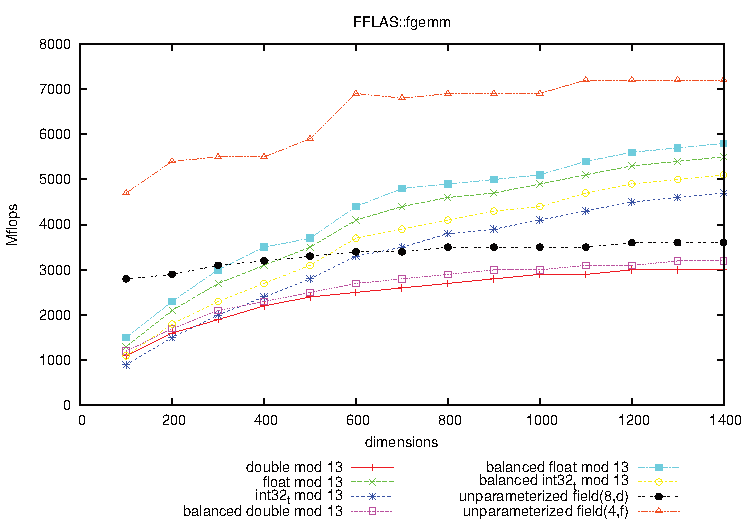
\includegraphics[scale=0.6]{Boyer_Brice/fgemm_square_13_ok}
	\caption{Example of \texttt{benchmark}: \texttt{fgemm}.\label{fig:bench}}
\end{figure}


%
% XXX Time spent on each data is limited (will not start execution if fit (linear least squares) forecasts 'too long'.\\
% XXX Adapts to the environment.
%
\subsection{Regression Testing}
%
Saving graphs in raw format can enable automatic regression testing on the
buildbots. For some determined matrices (of different shape and size) over a
few fields, we can accumulate over time the timings for some of our solutions
(rank, det, mul,\ldots). At each new release, when we update the documentation,
we can check any regression on these base cases and automatically update the
regression plots.
\danger We need to implement this framework (not difficult; anybody?).
%
\subsection{Method Selecting}
%
CPU throttling for ATLAS, \fflasffpack not reliable.
XXX Default are provided, method can be selected via a benchmark (cf wino\_threshold)\\
XXX howto

\section{Benchmarking  for automated tuning and regression testing}\label{sec:bench}
%
Benchmarking was introduced in \linbox for several reasons. First, It
gives the user a convenient way to produce quality graphs with the
help
of a graphing library like \gnuplot
\footnote{\url{http://www.gnuplot.info/}}
%
and provides the \linbox website with automatically updated tables and graphs.
Second, it can be used for regression testing.  Finally, it will be used for
selecting default methods and setting thresholds in installation time autotuning. % A lot of libraries do some automatic tuning
%at installation (\textsf{fftw}, \textsf{ATLAS}, \textsf{NTL},\ldots).
%
\par
%
% What do we do differently ? Selection between "larger" algorithms, takes more time.
% Interpolation.
% XXX BTL\footnote{\url{http://projects.opencascade.org/btl/}}/eigen
%
%
\subsection{Performance evaluation and Automated regression testing}
%
Our plotting mechanism is based on two structures: {\tt PlotStyle} and {\tt
PlotData}. The  {\tt PlotGraph} structure uses the style and data to manage the
output.  We allow plotting in standard image formats, html and \LaTeX tables,
but also in raw csv or xml for file exchange, data comparisons and
extrapolation.
%JGD: no comprendo
This mechanism can also automatically create benchmarks in \linbox
feature matrix (this is a table that describes what solutions we support, on
which the fields).
% \danger dave benchmark formats discussion ?
%
\par
%
% \begin{figure}[htbp]
	\centering
	\small
	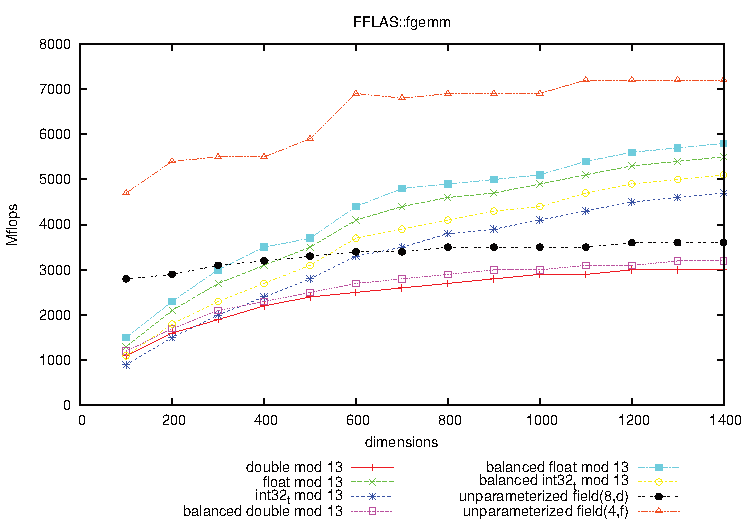
\includegraphics[scale=0.6]{Boyer_Brice/fgemm_square_13_ok}
	\caption{Example of \texttt{benchmark}: \texttt{fgemm}.\label{fig:bench}}
\end{figure}


%
% XXX Time spent on each data is limited (will not start execution if fit
% (linear least squares) forecasts 'too long'.\\
%
% XXX Adapts to the environment.
%
Saving graphs in raw format can also enable automatic regression testing on the
buildbots that already checked our code. For some specifically determined matrices (of
various shapes and sizes and over several fields), we can accumulate the timings
for key solutions such as ({\tt rank}, {\tt det}, {\tt mul},\ldots) over time.
At each new release, when the documentation is updated, we can check any
regression on these base cases and automatically update the regression plots.
% \danger We need to implement this framework (not difficult; anybody?).
%JGD: we already have the buildbot, lets focus on this right now
%
\subsection{Automated tuning and method selection}
%
Some of the code in \linbox is already automatically tuned (such as thresholds
in \fgemm), but we improve on it.
%It is well known that CPU throttling while
%building ATLAS causes bad optimizations; the \fflasffpack library could also
%suffer from not very reliable threshold detection (up to $50\%$ relative
%difference for some thresholds between runs).
Instead of searching for a
threshold using fast dichotomous techniques, for instance, we propose to
interpolate curves and find the intersection. Using least squares fitting, we
may even tolerate outliers (but this is time consuming).
%JGD: there is already optimizer/winograd.C etc.
%
\par
%
Automatically tuning a library is not only about thresholds, it may
also involve method/algorithm selection. Our strategy is the following: a given
algorithm is tuned for each {\tt Helper} (method) it has.  Then the solution
(that uses these algorithms) is tuned for selecting the best methods.  At each
stage, defaults are given, but can be overridden by the optimizer. The areas
where a method is better are extrapolated from the benchmark curves.
%
%
%%%%%%%%%%%%%%%%%%%%%%%%%%%%%%%
% Conclusion
%%%%%%%%%%%%%%%%%%%%%%%%%%%%%%%
%
%
% \input{Boyer_Brice/5-conclusion}
%
%
%%%%%%%%%%%%%%%%%%%%%%%%%%%%%%%
% Bib
%%%%%%%%%%%%%%%%%%%%%%%%%%%%%%%
%
%
\fi % abstractonly
% \bibliographystyle{abbrv}
% \bibliographystyle{acm}
% unComment either of the following:
% \bibliography{bboyer}
% %===== DO NOT MODIFY BEGIN============================
\documentclass[runningheads,a4paper]{llncs}
\usepackage{amssymb}
\setcounter{tocdepth}{3}
\usepackage{graphicx}
\usepackage{url}
\newcommand{\keywords}[1]{\par\addvspace\baselineskip
\noindent\keywordname\enspace\ignorespaces#1}
%===== DO NOT MODIFY END==============================
%%% packages
\clubpenalty 1000
\widowpenalty 1000

%%%%%%%%%%%%%%%%%%%%%%%%%%%%%%%
%%% Packages
%%%%%%%%%%%%%%%%%%%%%%%%%%%%%%%

\usepackage{iftex}
\usepackage{etex}
\usepackage{xspace}
\usepackage{setspace}

\ifXeTeX
%xetex
\fi

\ifLuaTeX
%luatex
\usepackage{fontspec}
\fi

\ifPDFTeX
% pdftex
\usepackage[utf8x]{inputenc}
\usepackage{lmodern}
\fi


\usepackage[english]{babel}
\usepackage{caption}
\usepackage{adforn}

\usepackage[x11names,svgnames]{xcolor}
% \usepackage{amsmath,amsthm,amsfonts,amssymb,graphicx}
% \usepackage{algorithm,%
%algorithmic%
% algpseudocode%
% }
\usepackage[%algochapter%
% ,linesnumbered%
,titlenumbered%
% ,vlined%
% ,lined%
,ruled%
% ,french%
% ,nofillcomment%
% ,onelanguage%
% ,scleft%
]{algorithm2e}
% \let\chapter\undefined % use this line

% FIXME numbersep>innerleftmargin, leftmargin=0.
\usepackage[%style=1
framemethod=%
TikZ
% PSTricks
% default
% ,skipbelow=-\topskip
% ,skipabove=\topskip
,nobreak=false
]{mdframed}

\usepackage{listings}

\usepackage[autolanguage]{numprint}

\usepackage{paralist,array,enumerate,multirow,float}% à moi
\usepackage[
breaklinks%
,colorlinks%
% ,linkcolor=red% internal document links
,linkcolor=MidnightBlue%
,anchorcolor=cyan%
%,pagecolor=blue%
,citecolor=blue%
,bookmarks=false%
]{hyperref}
\usepackage{url,xspace}
\usepackage{bm} %boldmath
\usepackage{booktabs}
\usepackage[%
% french%
]{cleveref}

\usepackage{stmaryrd}
\usepackage{tikz}

%%%%%%%%%%%%%%%%%%%%%%%%%%%%%%%
%%% to be removed packages
%%%%%%%%%%%%%%%%%%%%%%%%%%%%%%%
\usepackage{fourier-orns}
\usepackage{comment}

%%%%%%%%%%%%%%%%%%%%%%%%%%%%%%%
%%% Tuning
%%%%%%%%%%%%%%%%%%%%%%%%%%%%%%%
\usetikzlibrary{shapes,matrix,arrows}

\renewcommand\algomargin{1em} %double cadratin
%%% LISTINGS %%%
\mdfsetup{roundcorner=5%
,backgroundcolor=LightBlue!2!white%
,linecolor=LightBlue!60!black%
,leftmargin=0pt,rightmargin=0pt
,innerleftmargin=8pt,innerrightmargin=5pt
% ,innerleftmargin=15pt,innerrightmargin=5pt
,skipabove=\topskip
,skipbelow=-\topskip
% ,nobreak=false
}

\BeforeBeginEnvironment{lstlisting}%
{\begin{mdframed}[nobreak=false]
	% \NoAutoSpacing %french
	\vskip-0.4\baselineskip
}
\AfterEndEnvironment{lstlisting}{\end{mdframed}\vspace{1\baselineskip}\par\nobreak}
\def\ifempty#1{\def\temparg{#1}\ifx\temparg\empty}
\newcommand{\lstcapt}[2][]{%
\captionsetup*{type=lstlisting} %étoile pour virer les warnings
\vspace{-0.4\baselineskip}%
\ifempty{#1}%
\captionof{lstlisting}{#2}%
\else%
\captionof{lstlisting}[#1]{#2}%
\fi%
\vspace{0.5\baselineskip}%
\setlength{\parindent}{5mm}
\captionsetup*{type=""} %étoile pour virer les warnings
% XXX bug à la con. parindent est perdu par lstlinting ou autres
}

\lstset{language=C++%
,numbers=left%
,numberfirstline=false%
% ,numberfirstline=true%
,stepnumber=5
,firstnumber=1
,numberstyle=\tiny%
,numbersep=15pt%
% ,numbersep=0pt%
,numberbychapter=true%
,keywordstyle=\color{DarkGreen}\bfseries%
,showspaces=false%
,showstringspaces=false%
,numberblanklines=true%
,captionpos=b%
,literate={>>}{\ensuremath{>>}}1%
% ,literate={::}{::}1%
,basicstyle=\small\ttfamily%
% ,lineskip=-1pt%
% ,emph={inline}%
,emphstyle=\color{DarkRed}\bfseries%
,commentstyle=\ttfamily\color{gray}%
,rulecolor=\color{LightBlue!50}%
,breaklines=true%
,columns=fixed%
% ,stringstyle=\ttfamily%
% ,basicstyle=\small\fontfamily{LuxiMono}\selectfont%
% ,backgroundcolor=\color{LightBlue!5!white}%
% ,float
,belowskip=0em%\smallskipamount%
% ,aboveskip=\smallskipamount%
% ,aboveskip=\bigskipamount%
% ,belowskip=\bigskipamount%
% ,abovecaptionskip=1em%
% ,belowcaptionskip=-2em%
% ,framesep=5em
,upquote=false
% ,inputencoding=OT1
,extendedchars=true
,escapechar=¬
,basewidth=0.55em
}
% \def\lstlistingname{Code}
\captionsetup[lstlisting]{position=below}

%%%%%%%%%%%%%%%%%%%%%%%%%%%%%%%
%%% defs
%%%%%%%%%%%%%%%%%%%%%%%%%%%%%%%

\def\largesimpletilde{\adforn{19}}
\def\largetilde{\adforn{18}}
\def\frob#1#2{\left\langle#1, #2 \right\rangle}

\newcommand{\dbl}{\texttt{double}\xspace}
\newcommand{\flt}{\texttt{float}\xspace}

\def\Zb{\mathbf{Z}}
\def\modring#1{\ensuremath\Zb{/ #1\Zb}}
\def\gnuplot{\textsf{gnuplot}\xspace}



\newcolumntype{C}{>{$}c<{$}}
\newcolumntype{L}{>{$}l<{$}}
\newcolumntype{R}{>{$}r<{$}}


\def\linbox{\textsf{LinBox}\xspace}
\def\mul{\texttt{mul}\xspace}
\def\apply{\texttt{apply}\xspace}
\def\cpp{\textsf{C++}\xspace}
\def\mari{\textsf{m4ri}\xspace}
\def\fflas{\textsf{FFLAS}\xspace}
\def\fflaflas{\fflas}
\def\givaro{\textsf{Givaro}\xspace}
\def\applin{\textsf{BlackBox}\xspace}
\newcommand{\cf}{\mbox{\emph{cf.}}\xspace}
\newcommand{\eg}{\mbox{\emph{e.g.}}\xspace}
\newcommand{\ie}{\mbox{\emph{i.e.}}\xspace}
\def\mailto#1{\href{mailto:#1}{#1}}

%JGD
\makeatletter
\def\@fnsymbol#1{\ensuremath{\ifcase#1\or \natural \or
    \mathparagraph\or \dagger\or \ddagger\or \mathsection\or \nshortmid
    \or \dagger\dagger \or \ddagger\ddagger \or \sharp \or
   \nshortparallel \or \lightning \or \oint \or \daleth \or \gimel
   \or \clubsuit \or
   \spadesuit \or\hearsuit \or \diamondsuit \else\@ctrerr\fi}}
\makeatother
%===== DO NOT MODIFY BEGIN============================
\begin{document}

\mainmatter
%===== DO NOT MODIFY END==============================

%%%%%%%%%%%%%%%%%%%%%%%%%%%%%%%
%%% Title
%%%%%%%%%%%%%%%%%%%%%%%%%%%%%%%

\title{Elements of Design for Containers and Solutions in the \linbox library}
\subtitle{Extended abstract}
\titlerunning{Elements of Design for Containers and Solutions in the \linbox library}

\author{Brice Boyer\inst{1}%
%
\and Jean-Guillaume Dumas\inst{2}%
%
\and Pascal Giorgi\inst{3}%
%
\and Cl\'ement Pernet\inst{4}%
%
\and B. David Saunders\inst{5}%
 %
}
\authorrunning{Boyer--Dumas--Giorgi--Pernet--Saunders}%
% \authorrunning{B. Boyer, J-G. Dumas, P. Giorgi, C. Pernet, B. D. Saunders}


\institute{%
	\renewcommand{\thefootnote}{\fnsymbol{footnote}}
	Department of Mathematics, North Carolina State University,
	%Raleigh, NC,
	USA\footnote[2]{This material is based on work supported in part by
	the National Science Foundation under Grant CCF-1115772 (Kaltofen)}\\
	%
	\email{bbboyer@ncsu.edu}.
	%
	\and
	%
	Laboratoire J. Kuntzmann, Universit\'e de Grenoble.
	% 51, rue des Math\'ematiques, umr CNRS 5224, bp 53X, F38041 Grenoble,
        France\footnote[3]{This material is based on work supported in part by the
          Agence Nationale pour la Recherche under Grant
          ANR-11-BS02-013 HPAC (Dumas, Giorgi, Pernet).}\\
	%
	\email{Jean-Guillaume.Dumas@imag.fr}.
	%
	\and
	%
	% Laboratoire d'Informatique, de Robotique et de
	% Micro\'electronique de Montpellier (%
	LIRMM%
%)
	, CNRS, Universit\'e Montpellier 2,
	% 161 rue ADA, F-34095 Montpellier,
	France\footnotemark[3]\\
        %
        \email{pascal.giorgi@lirmm.fr.}
	%
	\and
	%
	Laboratoire LIG, Universit\'e de Grenoble et INRIA,
% umr CNRS, F38330 Montbonnot,
	France\footnotemark[3]\\
	%
	\email{clement.pernet@imag.fr}.
%
	\and
	%
	University of Delaware, Computer and Information Science Department,
	% Newark / DE / 19716,
	USA\\
	%
	\email{saunders@udel.edu}.%
	%
}


\date{}

\newif\ifAbstractOnly
% \AbstractOnlytrue
\AbstractOnlyfalse


\maketitle

\begin{abstract}
	%
	We develop in this paper design techniques used in the \cpp exact
	linear algebra library \linbox. They are intended to make the library
	safer and easier to use, while keeping it generic and efficient.
	%
	\par
	%
	First, we review the new simplified structure of the containers, based
	on our \emph{founding scope allocation} model.  Namely, vectors and
	matrix containers are all templated by a field and a storage type.
	Matrix interfaces all agree with the same minimal blackbox interface.
	This allows e.g. for a unification of our dense and sparse matrices, as
	well as a clearer model for matrices and submatrices. We explain the
	design choices and their impact on coding.	 We will describe
	serveral of the new containers, especially our sparse and dense
	matrices storages as well as their \apply (\emph{blackbox}) method and
	compare to previous implementations.%
	\par
	%
	Then we present a variation of the \emph{strategy} design pattern that
	is comprised of a controller--plugin system: the controller (solution)
	chooses among plug-ins (algorithms) and the plug-ins always call back
	the solution so a new choice can be made by the controller. We give
	examples using the solution \mul, and generalise this design pattern
	to the library. We also show performance comparisons with former \linbox
	versions.
	%
	\par
	%
	Finally we present a benchmark architecture that serves two purposes.
	The first one consists in providing the user with an easy way to
	produces graphs using \cpp. The second goal is to create a framework
	for automatically tuning the library (determine thresholds, choose
	algorithms) and provide a regression testing scheme.
	%
        \keywords{\linbox, design pattern, solutions and containers, benchmarking}
\end{abstract}


\ifAbstractOnly
% \ifdefined\doabstract
\else



%%%%%%%%%%%%%%%%%%%%%%%%%%%%%%%
% Intro
%%%%%%%%%%%%%%%%%%%%%%%%%%%%%%%
%
\section{Introduction}

The \linbox library is under constant evolution, driven by new problems and
algorithms, new compilers, new computing paradigms. This poses new challenges.
We are incrementally updating the design of the library towards a \textsf{2.0}
release.
%
\par
%
We show in the next \cref{tab:sloc} the increase in the size%
%
\footnote{Using \textsf{sloccount}, available at
\url{http://sourceforge.net/projects/sloccount/}.}
%
of \linbox.
%
\par
%
\begin{table}[htbp]
	\centering
	\caption[Evolution of the number of lines of codes in \linbox]{Evolution of the number of lines of code (loc, in thousands)
		in \linbox, \fflas and \givaro (\textdagger contains \givaro,
	\textdaggerdbl contains \fflaflas).}
	\label{tab:sloc}
	\begin{tabular}{rcccccccccc}
		\toprule
		\linbox & \sf 1.0.0\textsuperscript{\textdagger,\textdaggerdbl} & \sf 1.1.0\textsuperscript{\textdagger,\textdaggerdbl}& \sf 1.1.6\textsuperscript{\textdaggerdbl} & \sf 1.1.7\textsuperscript{\textdaggerdbl} & \sf 1.2.0 & \sf 1.2.2 & \sf 1.3.0 & \sf 1.4.0\\
		loc & {\numprint{77.3}}& {\numprint{85.8}} & {\numprint{93.5}} & {\numprint{103}} & {\numprint{108}}  & {\numprint{109}} &        {\numprint{112}} & \numprint{135} \\
		\midrule
		\fflaflas &N/A&N/A& N/A & \sf 1.3.3 & \sf 1.4.0 & \sf 1.4.3 & \sf 1.5.0 & \sf 1.8.0 \\
		loc & --- & ---& --- &\numprint{11.6} & {\numprint{23.9}} & {\numprint{25.2}} & {\numprint{25.5}} & \numprint{32.1}\\
		\midrule
		\givaro        & N/A& N/A & \sf 3.2.16        & \sf 3.3.3         &  \sf 3.4.3         & \sf 3.5.0         & \sf 3.6.0 & \sf 3.8.0 \\
		loc&---&---& \numprint{30.8} & {\numprint{33.6}}   & {\numprint{39.4}} & {\numprint{41.1}} & {\numprint{41.4}} &  \numprint{42.8} \\
		\midrule
		total  &  \numprint{77.3} & \numprint{85.8} & \numprint{124} & \numprint{137} & \numprint{171} & \numprint{175} & \numprint{179} & \numprint{210} \\
		\bottomrule
	\end{tabular}
\end{table}
%
The increase in the library size demands a stricter developpement model. For
instance, we have put \fflas files into a new stand-alone \fflas header
library, reduced compile times, enforced stricter warnings and checks, support
for more compilers and architectures, simplified and automatised version number
changes, automatised memory leak checks,\dots This demand on the developper
side is also driven by the fact that code introduced by various one-timers
needs to be maintained.
%
\par
%
But this increase also forces the library to be more user friendly. For
instance, we have: Developped an \texttt{auto-install.sh} script that installs
automatically the lastest stable or developpement versions of the trio;
Facilitated the discovery of the \textsc{Blas}/\textsc{Lapack} libraries;
Simplified and sped up the checking process; Added comprehensive benchmarking tools,\dots
%
\par
%
This article follows several papers and memoirs on \linbox
(\cite{Giorgi:2004:these,Turner:2002:these,Boyer:12,Dumas:2002:icms,Dumas:2010:lbpar})
and builds upon them.
%
\par
%
Developping generic and high-performance libraries is difficult. We can find a
large litterature on coding standards and software desin references in
(\cite{alexandrescu:01:modern,gamma:95:design,sutter:05:cpp,stroustrup1994design,Douglas:05:GPHP}),and  many internet sources and a lot of
experience acquired by free software projects.
%
\par
%
We are going to describe the advancement in the design of \linbox in the next
three sections. We will first describe the new \emph{container} framework in
\cref{sec:container}, then improve the \emph{matrix multiplication} algorithms
in \cref{sec:matmul} by contributing special purpose matrix multiplication
plugings, and finally present the new \emph{benchmark/optimisation}
architecture (\cref{sec:bench}).


%
%%%%%%%%%%%%%%%%%%%%%%%%%%%%%%%
% Containers
%%%%%%%%%%%%%%%%%%%%%%%%%%%%%%%
%
%
\section{Containers architecture}\label{sec:container}
%
\linbox is mainly conceived around the RAII concept with re-entrant function
(Resource Acquisition Is Initialisation), introduced by
\cite{stroustrup1994design}. We also follow the {founding scope allocation}
model (or \emph{mother model}) from \cite{Dumas:2010:lbpar} which ensures that
the memory used by objects is allocated in the constructor and freed only at
its destruction. The gestion of the memory allocated by an object is then
exlusively reserved to it.
%
\par
%
\linbox essentially uses matrix and vectors over fields and rings as data objects
(containers).  The fragmentation of the containers into various matrix and
blackbox types needed to be addressed and simplified. The many different matrix and
vector types with different interfaces needed to be reduced into only two
(possibly essentially one in the future) containers: \texttt{Matrix} and
\texttt{Vector}.
%
\subsection{General Interface for %Vectors and
Matrices}
%
First, in order to allow operations on its elements, a container is
parametrized by a field object (\cf \Cref{code:clmat}), not the field's element type. This simpler and 
more general.  The storage type is given by a second template parameter
that can default to \eg dense BLAS type matrices (a stride and a leading
dimension or an increment).  % what else can it be?
%
{
	\small
\begin{lstlisting}
template< class _Field, class _Storage = denseDefault >
class Vector ;
\end{lstlisting}
\lstcapt{Matrix and vector classes in \linbox.\label{code:clmat}}
}
% template< class _Field, class _Storage = denseDefault >
% class Matrix ;

%
In the mother model, we must distinguish containers that own (are responsible for allocated memory) and containers that share some
memory.  The \texttt{SubMatrix} and \texttt{SubVector} types share the memory
while \texttt{Matrix} and \texttt{Vector} own it.
%
The common interface shared by all matrices is the \applin  interface described
in the following paragraphs.
% \Cref{code:bb}.
%
% {
	\small
\begin{lstlisting}
template< ¬\ldots¬ >
class Matrix {
public:
        /* constructors */
	// no empty constructor
	// with a field, rows, columns, other matrix\dots

	/* y <- A.x or y <- A^T.x */
        template<class _in, class _out>
        _out& apply(_out &y, const _in &x) const;
        template<class _in, class _out>
        _out& applyTranspose(_out &y, const _in &x) const;

        /* operator rebind */
        template<typename _Tp1>
        struct rebind ;

        /* dimensions */
        size_t rowdim() const;
        size_t coldim() const;

        /* field */
        const Field& field() const;

	/* conversions */
	// resize
	// export/import to default types

	/* building the matrix */
	// read from MM/stdout/...
	// write to MM/stdout/...
	// setEntry/init()/finalise()/optimize()
protected:
        /* internals */
        ¬\ldots¬
};
\end{lstlisting}
\lstcapt{Interface of an \applin\label{code:bb}}
}
	% ¬\ldots¬
	% /* types */
	% // submatrix types
	% ¬\ldots¬

%
\begin{description}
%
	\item[Input/Output.] Our matrix all read and write from MatrixMarket
		format (ref, link).  Adding extra comments ? (for instance the
		{\tt init} field function in GF(q) needs a polynomial\ldots) We
		can adapt the hearder to suit our needs. In particular write
		matrix in CSR fashion (saving roughly 1/3 space over COO)
%
	\item[Accessing Elements.] The function \texttt{setEntry(...)} can be
		used to populate/grow the matrix (from some \texttt{init()}
		until a \texttt{finish()} is emitted).  The function
		\texttt{setEntry} can be (very) costly (for some sparse formats
		for instance) (Dave ?)
% so set entry should always build some COO or CSR and then
% convert to the format.
%
		\begin{itemize}
			%
			\item \texttt{refEntry} that retrieves a reference to
				an entry may be difficult to implement or
				inefficient (compressed fields, sparse
				matrices)
			%
			\item \texttt{getEntry} may be specialized, in all
				cases, there is a solution for this operation
				(can always be implemented from \texttt{imply},
				\cf{} later.
			%
			\item \texttt{clearEntry} can be used to zero out an
				entry, especially for a sparse matrix, if this
				is allowed (possibly not for structured
				matrices).
			%
			\item iterators may be difficult to implement (but a
				lot of code relies on them\ldots). Do we want
				only {\tt const} iterators ?
%
		\end{itemize}
%
	\item[Apply method.]
		This is essential in the \applin interface, and we'll described
		it in \Cref{ssec:apply,sec:matmul}.
%
	\item[Rebind] Rebind from one field to the other (if possible, using some default homeomorphism)
%
	\item[Other] Conversion mechanisms are added to the interface when
		convenient, for instance all sparse matrix formats can convert
		to/from CSR format. This `star' mechanism can simplify the code
		(to the expense of memory).
%
\end{description}
%
\subsection{The \texttt{apply} method}\label{ssec:apply}
%
% We will discuss the \texttt{apply} function in \Cref{sec:apply}.
% Both vec/mat
%
\par
%
The \texttt{apply} method (left or right) is arguably the most important
feature in the matrix interface and the \linbox library. It performs what a
linear application is defined for: apply to a vector (and by extension  a block
of vectors, \ie a matrix).
%
\par
%
We propose the new interface (\Cref{code:apply}), where {\tt \_In} and {\tt
\_Out} are vector or matrices, and {\tt Side} is either {\tt Tag::Right} or
{\tt Tag::Left}, wether the operation $y \gets A^{\top} x$ or  $y \gets A x$ is
performed.
%
{
\small
\begin{lstlisting}
// y = A.x
template< class _In, class _Out  >
_Out& apply(_Out &y, const _In& x, enum Side) ;

// y = alpha y + beta A.x
template< class _In, class _Out  >
_Out& applyAcc(_Out &y, const Element& alpha, const _In& x, const Element& beta, enum Side) ;

\end{lstlisting}
\lstcapt{Apply methods.\label{code:apply}}
}

%
This method is important for two reasons: first it is the building block of the
\applin algorithms (for instance Wiedemann and block-Wiedemann); second the
matrix multiplication is a basic operation in linear algebra that needs to be
extremely efficient (this is the matter of \Cref{sec:matmul}).
%
% The apply method should be using a \texttt{mul} solution as in the
% \Cref{code:applymul}.
%
%
\subsection{Examples of Containers}
%
First, we have the dense containers that follow some BLAS conventions (row
major ordering, leading dimension or increment,\ldots) and are based on {\tt
std::vector} (inheriting for instance the iterators). In the same fashion, we
have permutations matrices that follow the compressed \textsc{Lapack} format or
more traditional representations.
%
\par
%
We have many kinds of structured or compound matrices (Hankel, stacked, add, sub,\ldots)
All other matrices (including the special case of Permutations) : the same
Structured matrices, add, sub, stacked,\dots
%
\par
%
Finally, the sparse matrices are very important containers and require
particular interest because they are the basis of our \applin algorithms.
%
%
Sparse matrices are usually problematic because the notion of \emph{sparsity}
is too general \emph{vs.} the specificity of real world sparse matrices: the
algorithms have to adapt to the shape of the sparse matrices ---which is not really the case
for the dense case.
%
Getting the best performance for an sparse matrix as an \applin is not a
challenging task. There is a huge literature on \spmv (Sparse Matrix Vector
multiplication) and on sparse matrix formats, some of which are becoming
standard (COO, CSR, BCSR, SKY,\ldots).  In \cite{Boyer:2010:spmv} we developped
some techniques to improve the \spmv operation in \linbox.
Just like the \textsc{Blas} numerical
routines, we would also like to take advantage of existing high performance
numerical libraries (come back to this later).
%
\par
%
The addition of standard matrix format is driven by the availability of
numerical routines and the expectation of better performance in the \spmv
operation. However, legacy \linbox sparse matrix formats (based on STL
structures such as {\tt map}, {\tt deque}, {\tt pair},\ldots) can be more
convenient for elimination techniques.
%
%
\par
%
%XXX timing new matrices, example rank.
%
%

%
%
%%%%%%%%%%%%%%%%%%%%%%%%%%%%%%%
% Mat Mul
%%%%%%%%%%%%%%%%%%%%%%%%%%%%%%%
%
%
\section{Improving \linbox matrix multiplication}\label{sec:matmul}
%
We propose a \emph{design pattern} (the closest pattern to our knowledge is the
\emph{strategy} one, see \cite[Fig 2.]{Cung:2006:TC}) in \Cref{ssec:plugin} and
we show a variety of new algorithms where it is used in the \mul  solution
(\Cref{ssec:algmul}).
%
\subsection{Plugin structure}\label{ssec:plugin}
%
We propose the following version of the \emph{strategy design pattern}, 
see \cite[Fig 2.]{Cung:2006:TC}).
The main advantage of this pattern is that the modules always call 
the controller of a function so that the best version will be chosen. 
% Besides modules can be easily added as \emph{plugins}.
An analogy can be drawn with dynamic
\begin{wrapfigure}{r}{0.42\textwidth}
% \begin{figure}[htbp]
	\vspace{-2.2em}
	\begin{center}
	\small
\tikzstyle{block} = [draw, fill=blue!20, rectangle,
    minimum height=1.7em, minimum width=5.5em, rounded corners]
\tikzstyle{input} = [coordinate]
\tikzstyle{output} = [coordinate]
\tikzstyle{fleche} = [draw,->,shorten <=3pt, shorten >=3pt,thick]
% \tikzstyle{pinstyle} = [pin edge={to-,thin,black}]
	% \centering
\begin{tikzpicture}[auto, node distance=2.0cm,>=latex']
        \node [input, name=input] (input) {};
        \node [block, right of=input] (controller) {Controlers};
        \node [output, right of=controller] (output) {};

        \node [block, below of=controller] (modules) {Modules};

        \draw [fleche] (input) to [near start] node {input} (controller);
        \draw [fleche] (controller) to [near end] node {output} (output);
        \draw [fleche] (controller.300) to [bend left,near end] node [right] {call} (modules.60);
        \draw [fleche] (modules.120) to [bend left,near end] node [left] {call back} (controller.240);
\end{tikzpicture}
	% \vspace{-1em}
\caption{Controller/Module design pattern}
\end{center}
\label{fig:diag:patt}
	\vspace{-2.2em}
% \end{figure}
\end{wrapfigure}

systems --- once the controller sends a correction to the system, it receives
back a new measure that allows for a new correction.
%
\par
%
%
%
%
For instance, we can write (\Cref{fig:seuil}) the standard cascade algorithms
(see \cite{Dumas:2008:Flas}) in that model. Cascade algorithms are used to combine
several algorithms that are switched using thresholds, ensuring better
efficiency than that of any of the algorithms individually.
%
% \par
%
%
This method allows for the reuse of modules and ensures efficiency.
It is then possible to adapt to the architecture, the available modules,
the resources. The only limitation is that the choice of module
must be fast.
%
% \par
%
On top of this design, we have Method objects that allow caller selection
of preferred algorithms, shortcutting the strategy selection.
%
\begin{figure}[htbp]
	\small
        \hfil
        \begin{minipage}{0.47\textwidth}
                \begin{algorithm}[H]
                        \caption{\texttt{Algo}: controler}
                        \label{alg:controle}
                        \KwIn{$A$ and $B$, denses, with resp. dimensions $n\times
                        k$ and $k\times n$.}
			\KwIn{$H$ Helper}
                        \KwOut{$C = A\times B$}
			\eIf{$\mathrm{min}(m,k,n)<H.{\tt threshold}()$}{
				{\tt BaseCase} K() ; \\
				{\tt Algo}(C,A,B,K) ; %\tcc{\small{\color{gray}fast BLAS}}
			}
			{
				{\tt RecursiveCase} H() ; \\
				{\tt Algo}(C,A,B,H)
			}
                        \KwRet C \;
                \end{algorithm}
        \end{minipage}
        \hfil
        \begin{minipage}{0.47\textwidth}
                \begin{algorithm}[H]
                        \DontPrintSemicolon
                        \caption{\texttt{Algo}: recursive module}
                        \label{alg:action}
                        \KwIn{$A$, $B$, $C$ as in controller.}
			\KwIn{$H$, {\tt RecursiveCase} Helper}
                        \KwOut{$C = A\times B$}
                        Cuts $A$,$B$,$C$ in $S_i, T_i\cdots$\;
                        \ldots \;
                        $P_i = \mathtt{Algo}(S_i,T_i,H)$ \;
                        \ldots \;
                        \KwRet C \;
                \end{algorithm}
        \end{minipage}
        \hfil
        \caption{Conception of a recursive controlled algorithm}
        \label{fig:seuil}
\end{figure}

% \par
%
% \danger timing old fgemm/plugin fgemm with no noticeable change ?
%
\par
%
This infrastructure supports modular code. For instance,
\fflasffpack has seen major  modularization (addition, scaling,
reduction,\ldots) Not only does it enable code to be hardly longer than
the corresponding pseudocode listings, \cite{Boyer:2009:sched}, (compared to
$\approx 2.5\times$ on some routines before) but it also automatically brings
performance, because we can separately improve individual modules and immediately have the benefit throughout the library.
%% following could be in, but perhaps cut now for reducing to 8 pages
%Also, this reduces the lines of code, hence the
%probability for bugs, eases their tracing/tracking, and allows for more
%unit tests. Modularizing the code comes at almost no cost because we may add
%$O(1)$  operations that: Do not cost much compared to $O(n^2)$ or more
%complexity of the modules; Allow early decisions and terminations (\eg by
%testing against $0$, $\pm 1$, checking leading dimensions or increments);
%Allow better code (AVX, SSE, copy--cache friendly operation--copy back,
%representation switching,\ldots)
%
\subsection{New algorithms for the \mul solution}\label{ssec:algmul}
%
New algorithms and techniques improve on matrix multiplication
in several  ways: reducing memory consumption, reducing runtime, 
using graphics capabilities, generalizing the BLAS to integer
routines.
%
\def\monitem#1{\par \textit{#1}\ }
\monitem{Reduced memory.}
%
The routine \fgemm in \fflas uses by default the classic schedules for the multiplication
and the product with accumulation (\cf \cite{Boyer:2009:sched}), but we also
implement the low memory routines therein. The new algorithms are competitive
and can reach sizes that were limiting.
%
% \par
%
One difficulty consists in using the memory contained in a submatrix of
the original matrix, that one cannot free or reallocate.
%
\monitem{Using Bini's approximate formula.}
%
In \cite{BD:2014:Bini}, we use Bini's approximate matrix multiplication formula
to derive a new algorithms that is more efficient that the Strassen--Winograd
implementation in \fgemm by $\approx 5-10\%$ on sizes \num{1500}--\num{3000}.
This is a cascade of Bini's algorithm and Strassen--Winograd algorithm and/or
the naïve algorithm (using BLAS). The idea is to analyze precisely the error
term in the approximate formula and make it vanish.
%
\monitem{Integer BLAS.}
%
In order to provide fast matrix multiplication with multiprecision integers, we
rely on multimodular approach through the Chinese remainder theorem. Our
approach is to reduce as much as possible to \fgemm. Despite, the existence of
fast multimodular reduction (resp.\ reconstruction) algorithm
\cite{VonzurGathen:1999:MCA}, the naive quadratic approach can be reduced to
\fgemm which makes it more efficient into practice.  Note that providing
optimized fast multimodular reduction remains challenging. This code is
directly integrated  into \fflas.

%
\monitem{Polynomial Matrix Multiplication over small prime fields.}
%
The situation is similar to integer matrices since one can use
evaluation/interpolation techniques through DFT transforms. However, the
optimized Fast Fourier Transform of \cite{Harvey:2014}  makes fast evaluation
(resp.\ interpolation) competitive into practice. We thus rely on this scheme
together with \fgemm for pointwise matrix multiplications. One can find some
benchmark of our code in \cite{GioLeb14}.
%
\monitem{Sparse Matrix--Vector Multiplication}
%
Sparse matrices are usually problematic because the notion of \emph{sparsity}
is too general \vs the specificity of real world sparse matrices: the
algorithms have to adapt to the shape of the sparse matrices.
%
There is a huge literature from numerical linear algebra  on \spmv (Sparse
Matrix Vector multiplication) and on sparse matrix formats, some of which are
becoming standard (COO, CSR, BCSR, SKY,\ldots).  In \cite{Boyer:2010:spmv} we
developed some techniques to improve the \spmv operation in \linbox. Ideas
include the separation of the $\pm 1$ for removing multiplications, splitting
in a sum (HYB for hybrid format) of sparse matrix  whose formats are
independent and using specific routines. For instance, on $\modring{p}$ with
word size $p$, one can split the matrix ensuring no reduction is needed  in the
dot product and call Sparse BLAS (from Intel \textsf{MKL} or Nvidia
\textsf{cuBLAS} for instance) on each matrix. One tradeoff is as usual between
available memory, time spent on optimizing \vs time spent on \apply, and all
the more so because we allow the concurrent storage of the transpose in an
optimized fashion, usually yielding huge speedups. This can be decided by
\emph{ad hoc.\ } optimizers.
% Helper structure to store a matrix as a sum of structures (HYB), possibly the
%
%\monitem{Parallelization}
Work on parallelizations using \textsf{OpenCL}, \textsf{OpenMP} or
\textsf{XKaapi} for dense or sparse matrix multiplication include
\cite{Boyer:2010:spmv,WST12,DGPZ14}.

\begin{comment} % taken for length reduction
\paragraph{}
These state-of-the-art algorithms, often interdependent, need to be selected
by the \mul solution, possibly using a Method/Helper parameter. The
Controller/Module model works particularly well here: cascading, switch
methods, algorithms selection is made easy. Besides, the choosing of a
particular algorithms or base case is never settled in advance: the library has
to be tuned wrt. available libraries, local performance of these libraries.
\end{comment}

\begin{comment}
\monitem{Using conversions}
\begin{itemize}
	\item
 double->float
	\item
 using flint for integer matmul is faster, even with conversion. Need better CRA implementation (but with the plugins, we can do without our faulty code and just use flint).
	\item
 implementation of Toom-Cook for GF(q)
	\item
 when does spmv choose to optimize ?
	\item
 transition to benchmarking
\end{itemize}
%
\danger dave some words on the Domain architecture that you support and why it is best than functions (for instance for mul or apply) ?
\end{comment}


%
%%%%%%%%%%%%%%%%%%%%%%%%%%%%%%%
% Bench
%%%%%%%%%%%%%%%%%%%%%%%%%%%%%%%
\section{Benchmarking}\label{sec:bench}
%
Benchmarking was introduced in \linbox for several reasons. First, It would
give the user a user-friendly way for producing quality graph with no necessary
knowledge of a graphing library like \gnuplot%
%
%
\footnote{\url{http://www.gnuplot.info/}}
%
or provide the \linbox website with automatically updated tables and graphs.
Second, it would be used for regression testing.  Finally, it would be used for
selecting default method, threshold. A lot of libraries do some automatic tuning
at installation (fftw, ATLAS, NTL,\ldots).
%
\par
%
What do we do differently ? Selection between "larger" algorithms, takes more time.
Interpolation.
% XXX BTL\footnote{\url{http://projects.opencascade.org/btl/}}/eigen
%
%
\subsection{Graph/Table creation}
%
Our plotting mechanism is based on two structures: {\tt PlotStyle} and {\tt
PlotData}. The  {\tt PlotGraph} structure uses the style and data to manage the
output.  We allow ploting in standard image formats, html and \LaTeX tables,
but also in raw csv or xml. The last raw formats allow for file exchange, data
comparisons and extrapolation.
\danger dave benchmark formats discussion ?
%
\par
%
% \begin{figure}[htbp]
	\centering
	\small
	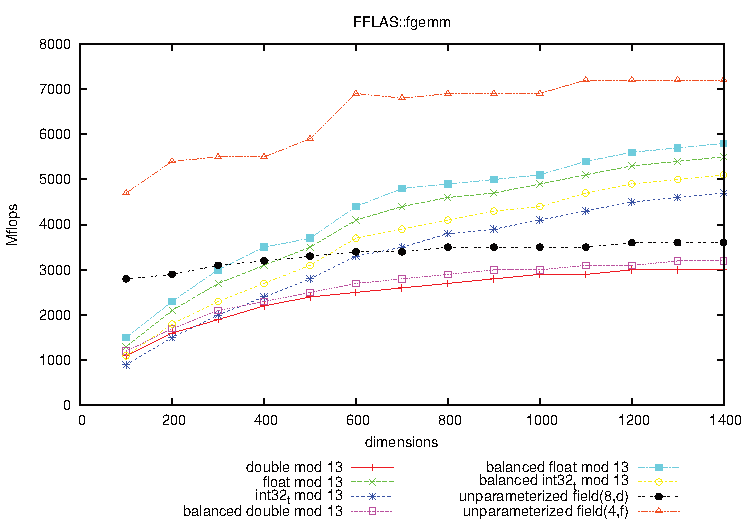
\includegraphics[scale=0.6]{Boyer_Brice/fgemm_square_13_ok}
	\caption{Example of \texttt{benchmark}: \texttt{fgemm}.\label{fig:bench}}
\end{figure}


%
% XXX Time spent on each data is limited (will not start execution if fit (linear least squares) forecasts 'too long'.\\
% XXX Adapts to the environment.
%
\subsection{Regression Testing}
%
Saving graphs in raw format can enable automatic regression testing on the
buildbots. For some determined matrices (of different shape and size) over a
few fields, we can accumulate over time the timings for some of our solutions
(rank, det, mul,\ldots). At each new release, when we update the documentation,
we can check any regression on these base cases and automatically update the
regression plots.
\danger We need to implement this framework (not difficult; anybody?).
%
\subsection{Method Selecting}
%
CPU throttling for ATLAS, \fflasffpack not reliable.
XXX Default are provided, method can be selected via a benchmark (cf wino\_threshold)\\
XXX howto

%
%
%%%%%%%%%%%%%%%%%%%%%%%%%%%%%%%
% Conclusion
%%%%%%%%%%%%%%%%%%%%%%%%%%%%%%%
%
%
\input{5-conclusion}
%
%
%%%%%%%%%%%%%%%%%%%%%%%%%%%%%%%
% Bib
%%%%%%%%%%%%%%%%%%%%%%%%%%%%%%%
%
%
\fi % abstractonly

\bibliographystyle{abbrv}
% \bibliographystyle{acm}
\bibliography{bboyer}
% %===== DO NOT MODIFY BEGIN============================
\documentclass[runningheads,a4paper]{llncs}
\usepackage{amssymb}
\setcounter{tocdepth}{3}
\usepackage{graphicx}
\usepackage{url}
\newcommand{\keywords}[1]{\par\addvspace\baselineskip
\noindent\keywordname\enspace\ignorespaces#1}
%===== DO NOT MODIFY END==============================
%%% packages
\clubpenalty 1000
\widowpenalty 1000

%%%%%%%%%%%%%%%%%%%%%%%%%%%%%%%
%%% Packages
%%%%%%%%%%%%%%%%%%%%%%%%%%%%%%%

\usepackage{iftex}
\usepackage{etex}
\usepackage{xspace}
\usepackage{setspace}

\ifXeTeX
%xetex
\fi

\ifLuaTeX
%luatex
\usepackage{fontspec}
\fi

\ifPDFTeX
% pdftex
\usepackage[utf8x]{inputenc}
\usepackage{lmodern}
\fi


\usepackage[english]{babel}
\usepackage{caption}
\usepackage{adforn}

\usepackage[x11names,svgnames]{xcolor}
% \usepackage{amsmath,amsthm,amsfonts,amssymb,graphicx}
% \usepackage{algorithm,%
%algorithmic%
% algpseudocode%
% }
\usepackage[%algochapter%
% ,linesnumbered%
,titlenumbered%
% ,vlined%
% ,lined%
,ruled%
% ,french%
% ,nofillcomment%
% ,onelanguage%
% ,scleft%
]{algorithm2e}
% \let\chapter\undefined % use this line

% FIXME numbersep>innerleftmargin, leftmargin=0.
\usepackage[%style=1
framemethod=%
TikZ
% PSTricks
% default
% ,skipbelow=-\topskip
% ,skipabove=\topskip
,nobreak=false
]{mdframed}

\usepackage{listings}

\usepackage[autolanguage]{numprint}

\usepackage{paralist,array,enumerate,multirow,float}% à moi
\usepackage[
breaklinks%
,colorlinks%
% ,linkcolor=red% internal document links
,linkcolor=MidnightBlue%
,anchorcolor=cyan%
%,pagecolor=blue%
,citecolor=blue%
,bookmarks=false%
]{hyperref}
\usepackage{url,xspace}
\usepackage{bm} %boldmath
\usepackage{booktabs}
\usepackage[%
% french%
]{cleveref}

\usepackage{stmaryrd}
\usepackage{tikz}

%%%%%%%%%%%%%%%%%%%%%%%%%%%%%%%
%%% to be removed packages
%%%%%%%%%%%%%%%%%%%%%%%%%%%%%%%
\usepackage{fourier-orns}
\usepackage{comment}

%%%%%%%%%%%%%%%%%%%%%%%%%%%%%%%
%%% Tuning
%%%%%%%%%%%%%%%%%%%%%%%%%%%%%%%
\usetikzlibrary{shapes,matrix,arrows}

\renewcommand\algomargin{1em} %double cadratin
%%% LISTINGS %%%
\mdfsetup{roundcorner=5%
,backgroundcolor=LightBlue!2!white%
,linecolor=LightBlue!60!black%
,leftmargin=0pt,rightmargin=0pt
,innerleftmargin=8pt,innerrightmargin=5pt
% ,innerleftmargin=15pt,innerrightmargin=5pt
,skipabove=\topskip
,skipbelow=-\topskip
% ,nobreak=false
}

\BeforeBeginEnvironment{lstlisting}%
{\begin{mdframed}[nobreak=false]
	% \NoAutoSpacing %french
	\vskip-0.4\baselineskip
}
\AfterEndEnvironment{lstlisting}{\end{mdframed}\vspace{1\baselineskip}\par\nobreak}
\def\ifempty#1{\def\temparg{#1}\ifx\temparg\empty}
\newcommand{\lstcapt}[2][]{%
\captionsetup*{type=lstlisting} %étoile pour virer les warnings
\vspace{-0.4\baselineskip}%
\ifempty{#1}%
\captionof{lstlisting}{#2}%
\else%
\captionof{lstlisting}[#1]{#2}%
\fi%
\vspace{0.5\baselineskip}%
\setlength{\parindent}{5mm}
\captionsetup*{type=""} %étoile pour virer les warnings
% XXX bug à la con. parindent est perdu par lstlinting ou autres
}

\lstset{language=C++%
,numbers=left%
,numberfirstline=false%
% ,numberfirstline=true%
,stepnumber=5
,firstnumber=1
,numberstyle=\tiny%
,numbersep=15pt%
% ,numbersep=0pt%
,numberbychapter=true%
,keywordstyle=\color{DarkGreen}\bfseries%
,showspaces=false%
,showstringspaces=false%
,numberblanklines=true%
,captionpos=b%
,literate={>>}{\ensuremath{>>}}1%
% ,literate={::}{::}1%
,basicstyle=\small\ttfamily%
% ,lineskip=-1pt%
% ,emph={inline}%
,emphstyle=\color{DarkRed}\bfseries%
,commentstyle=\ttfamily\color{gray}%
,rulecolor=\color{LightBlue!50}%
,breaklines=true%
,columns=fixed%
% ,stringstyle=\ttfamily%
% ,basicstyle=\small\fontfamily{LuxiMono}\selectfont%
% ,backgroundcolor=\color{LightBlue!5!white}%
% ,float
,belowskip=0em%\smallskipamount%
% ,aboveskip=\smallskipamount%
% ,aboveskip=\bigskipamount%
% ,belowskip=\bigskipamount%
% ,abovecaptionskip=1em%
% ,belowcaptionskip=-2em%
% ,framesep=5em
,upquote=false
% ,inputencoding=OT1
,extendedchars=true
,escapechar=¬
,basewidth=0.55em
}
% \def\lstlistingname{Code}
\captionsetup[lstlisting]{position=below}

%%%%%%%%%%%%%%%%%%%%%%%%%%%%%%%
%%% defs
%%%%%%%%%%%%%%%%%%%%%%%%%%%%%%%

\def\largesimpletilde{\adforn{19}}
\def\largetilde{\adforn{18}}
\def\frob#1#2{\left\langle#1, #2 \right\rangle}

\newcommand{\dbl}{\texttt{double}\xspace}
\newcommand{\flt}{\texttt{float}\xspace}

\def\Zb{\mathbf{Z}}
\def\modring#1{\ensuremath\Zb{/ #1\Zb}}
\def\gnuplot{\textsf{gnuplot}\xspace}



\newcolumntype{C}{>{$}c<{$}}
\newcolumntype{L}{>{$}l<{$}}
\newcolumntype{R}{>{$}r<{$}}


\def\linbox{\textsf{LinBox}\xspace}
\def\mul{\texttt{mul}\xspace}
\def\apply{\texttt{apply}\xspace}
\def\cpp{\textsf{C++}\xspace}
\def\mari{\textsf{m4ri}\xspace}
\def\fflas{\textsf{FFLAS}\xspace}
\def\fflaflas{\fflas}
\def\givaro{\textsf{Givaro}\xspace}
\def\applin{\textsf{BlackBox}\xspace}
\newcommand{\cf}{\mbox{\emph{cf.}}\xspace}
\newcommand{\eg}{\mbox{\emph{e.g.}}\xspace}
\newcommand{\ie}{\mbox{\emph{i.e.}}\xspace}
\def\mailto#1{\href{mailto:#1}{#1}}

%JGD
\makeatletter
\def\@fnsymbol#1{\ensuremath{\ifcase#1\or \natural \or
    \mathparagraph\or \dagger\or \ddagger\or \mathsection\or \nshortmid
    \or \dagger\dagger \or \ddagger\ddagger \or \sharp \or
   \nshortparallel \or \lightning \or \oint \or \daleth \or \gimel
   \or \clubsuit \or
   \spadesuit \or\hearsuit \or \diamondsuit \else\@ctrerr\fi}}
\makeatother
%===== DO NOT MODIFY BEGIN============================
\begin{document}

\mainmatter
%===== DO NOT MODIFY END==============================

%%%%%%%%%%%%%%%%%%%%%%%%%%%%%%%
%%% Title
%%%%%%%%%%%%%%%%%%%%%%%%%%%%%%%

\title{Elements of Design for Containers and Solutions in the \linbox library}
\subtitle{Extended abstract}
\titlerunning{Elements of Design for Containers and Solutions in the \linbox library}

\author{Brice Boyer\inst{1}%
%
\and Jean-Guillaume Dumas\inst{2}%
%
\and Pascal Giorgi\inst{3}%
%
\and Cl\'ement Pernet\inst{4}%
%
\and B. David Saunders\inst{5}%
 %
}
\authorrunning{Boyer--Dumas--Giorgi--Pernet--Saunders}%
% \authorrunning{B. Boyer, J-G. Dumas, P. Giorgi, C. Pernet, B. D. Saunders}


\institute{%
	\renewcommand{\thefootnote}{\fnsymbol{footnote}}
	Department of Mathematics, North Carolina State University,
	%Raleigh, NC,
	USA\footnote[2]{This material is based on work supported in part by
	the National Science Foundation under Grant CCF-1115772 (Kaltofen)}\\
	%
	\email{bbboyer@ncsu.edu}.
	%
	\and
	%
	Laboratoire J. Kuntzmann, Universit\'e de Grenoble.
	% 51, rue des Math\'ematiques, umr CNRS 5224, bp 53X, F38041 Grenoble,
        France\footnote[3]{This material is based on work supported in part by the
          Agence Nationale pour la Recherche under Grant
          ANR-11-BS02-013 HPAC (Dumas, Giorgi, Pernet).}\\
	%
	\email{Jean-Guillaume.Dumas@imag.fr}.
	%
	\and
	%
	% Laboratoire d'Informatique, de Robotique et de
	% Micro\'electronique de Montpellier (%
	LIRMM%
%)
	, CNRS, Universit\'e Montpellier 2,
	% 161 rue ADA, F-34095 Montpellier,
	France\footnotemark[3]\\
        %
        \email{pascal.giorgi@lirmm.fr.}
	%
	\and
	%
	Laboratoire LIG, Universit\'e de Grenoble et INRIA,
% umr CNRS, F38330 Montbonnot,
	France\footnotemark[3]\\
	%
	\email{clement.pernet@imag.fr}.
%
	\and
	%
	University of Delaware, Computer and Information Science Department,
	% Newark / DE / 19716,
	USA\\
	%
	\email{saunders@udel.edu}.%
	%
}


\date{}

\newif\ifAbstractOnly
% \AbstractOnlytrue
\AbstractOnlyfalse


\maketitle

\begin{abstract}
	%
	We develop in this paper design techniques used in the \cpp exact
	linear algebra library \linbox. They are intended to make the library
	safer and easier to use, while keeping it generic and efficient.
	%
	\par
	%
	First, we review the new simplified structure of the containers, based
	on our \emph{founding scope allocation} model.  Namely, vectors and
	matrix containers are all templated by a field and a storage type.
	Matrix interfaces all agree with the same minimal blackbox interface.
	This allows e.g. for a unification of our dense and sparse matrices, as
	well as a clearer model for matrices and submatrices. We explain the
	design choices and their impact on coding.	 We will describe
	serveral of the new containers, especially our sparse and dense
	matrices storages as well as their \apply (\emph{blackbox}) method and
	compare to previous implementations.%
	\par
	%
	Then we present a variation of the \emph{strategy} design pattern that
	is comprised of a controller--plugin system: the controller (solution)
	chooses among plug-ins (algorithms) and the plug-ins always call back
	the solution so a new choice can be made by the controller. We give
	examples using the solution \mul, and generalise this design pattern
	to the library. We also show performance comparisons with former \linbox
	versions.
	%
	\par
	%
	Finally we present a benchmark architecture that serves two purposes.
	The first one consists in providing the user with an easy way to
	produces graphs using \cpp. The second goal is to create a framework
	for automatically tuning the library (determine thresholds, choose
	algorithms) and provide a regression testing scheme.
	%
        \keywords{\linbox, design pattern, solutions and containers, benchmarking}
\end{abstract}


\ifAbstractOnly
% \ifdefined\doabstract
\else



%%%%%%%%%%%%%%%%%%%%%%%%%%%%%%%
% Intro
%%%%%%%%%%%%%%%%%%%%%%%%%%%%%%%
%
\section{Introduction}

The \linbox library is under constant evolution, driven by new problems and
algorithms, new compilers, new computing paradigms. This poses new challenges.
We are incrementally updating the design of the library towards a \textsf{2.0}
release.
%
\par
%
We show in the next \cref{tab:sloc} the increase in the size%
%
\footnote{Using \textsf{sloccount}, available at
\url{http://sourceforge.net/projects/sloccount/}.}
%
of \linbox.
%
\par
%
\begin{table}[htbp]
	\centering
	\caption[Evolution of the number of lines of codes in \linbox]{Evolution of the number of lines of code (loc, in thousands)
		in \linbox, \fflas and \givaro (\textdagger contains \givaro,
	\textdaggerdbl contains \fflaflas).}
	\label{tab:sloc}
	\begin{tabular}{rcccccccccc}
		\toprule
		\linbox & \sf 1.0.0\textsuperscript{\textdagger,\textdaggerdbl} & \sf 1.1.0\textsuperscript{\textdagger,\textdaggerdbl}& \sf 1.1.6\textsuperscript{\textdaggerdbl} & \sf 1.1.7\textsuperscript{\textdaggerdbl} & \sf 1.2.0 & \sf 1.2.2 & \sf 1.3.0 & \sf 1.4.0\\
		loc & {\numprint{77.3}}& {\numprint{85.8}} & {\numprint{93.5}} & {\numprint{103}} & {\numprint{108}}  & {\numprint{109}} &        {\numprint{112}} & \numprint{135} \\
		\midrule
		\fflaflas &N/A&N/A& N/A & \sf 1.3.3 & \sf 1.4.0 & \sf 1.4.3 & \sf 1.5.0 & \sf 1.8.0 \\
		loc & --- & ---& --- &\numprint{11.6} & {\numprint{23.9}} & {\numprint{25.2}} & {\numprint{25.5}} & \numprint{32.1}\\
		\midrule
		\givaro        & N/A& N/A & \sf 3.2.16        & \sf 3.3.3         &  \sf 3.4.3         & \sf 3.5.0         & \sf 3.6.0 & \sf 3.8.0 \\
		loc&---&---& \numprint{30.8} & {\numprint{33.6}}   & {\numprint{39.4}} & {\numprint{41.1}} & {\numprint{41.4}} &  \numprint{42.8} \\
		\midrule
		total  &  \numprint{77.3} & \numprint{85.8} & \numprint{124} & \numprint{137} & \numprint{171} & \numprint{175} & \numprint{179} & \numprint{210} \\
		\bottomrule
	\end{tabular}
\end{table}
%
The increase in the library size demands a stricter developpement model. For
instance, we have put \fflas files into a new stand-alone \fflas header
library, reduced compile times, enforced stricter warnings and checks, support
for more compilers and architectures, simplified and automatised version number
changes, automatised memory leak checks,\dots This demand on the developper
side is also driven by the fact that code introduced by various one-timers
needs to be maintained.
%
\par
%
But this increase also forces the library to be more user friendly. For
instance, we have: Developped an \texttt{auto-install.sh} script that installs
automatically the lastest stable or developpement versions of the trio;
Facilitated the discovery of the \textsc{Blas}/\textsc{Lapack} libraries;
Simplified and sped up the checking process; Added comprehensive benchmarking tools,\dots
%
\par
%
This article follows several papers and memoirs on \linbox
(\cite{Giorgi:2004:these,Turner:2002:these,Boyer:12,Dumas:2002:icms,Dumas:2010:lbpar})
and builds upon them.
%
\par
%
Developping generic and high-performance libraries is difficult. We can find a
large litterature on coding standards and software desin references in
(\cite{alexandrescu:01:modern,gamma:95:design,sutter:05:cpp,stroustrup1994design,Douglas:05:GPHP}),and  many internet sources and a lot of
experience acquired by free software projects.
%
\par
%
We are going to describe the advancement in the design of \linbox in the next
three sections. We will first describe the new \emph{container} framework in
\cref{sec:container}, then improve the \emph{matrix multiplication} algorithms
in \cref{sec:matmul} by contributing special purpose matrix multiplication
plugings, and finally present the new \emph{benchmark/optimisation}
architecture (\cref{sec:bench}).


%
%%%%%%%%%%%%%%%%%%%%%%%%%%%%%%%
% Containers
%%%%%%%%%%%%%%%%%%%%%%%%%%%%%%%
%
%
\section{Containers architecture}\label{sec:container}
%
\linbox is mainly conceived around the RAII concept with re-entrant function
(Resource Acquisition Is Initialisation), introduced by
\cite{stroustrup1994design}. We also follow the {founding scope allocation}
model (or \emph{mother model}) from \cite{Dumas:2010:lbpar} which ensures that
the memory used by objects is allocated in the constructor and freed only at
its destruction. The gestion of the memory allocated by an object is then
exlusively reserved to it.
%
\par
%
\linbox essentially uses matrix and vectors over fields and rings as data objects
(containers).  The fragmentation of the containers into various matrix and
blackbox types needed to be addressed and simplified. The many different matrix and
vector types with different interfaces needed to be reduced into only two
(possibly essentially one in the future) containers: \texttt{Matrix} and
\texttt{Vector}.
%
\subsection{General Interface for %Vectors and
Matrices}
%
First, in order to allow operations on its elements, a container is
parametrized by a field object (\cf \Cref{code:clmat}), not the field's element type. This simpler and 
more general.  The storage type is given by a second template parameter
that can default to \eg dense BLAS type matrices (a stride and a leading
dimension or an increment).  % what else can it be?
%
\input{lst_container}
%
In the mother model, we must distinguish containers that own (are responsible for allocated memory) and containers that share some
memory.  The \texttt{SubMatrix} and \texttt{SubVector} types share the memory
while \texttt{Matrix} and \texttt{Vector} own it.
%
The common interface shared by all matrices is the \applin  interface described
in the following paragraphs.
% \Cref{code:bb}.
%
% \input{lst_applin}
%
\begin{description}
%
	\item[Input/Output.] Our matrix all read and write from MatrixMarket
		format (ref, link).  Adding extra comments ? (for instance the
		{\tt init} field function in GF(q) needs a polynomial\ldots) We
		can adapt the hearder to suit our needs. In particular write
		matrix in CSR fashion (saving roughly 1/3 space over COO)
%
	\item[Accessing Elements.] The function \texttt{setEntry(...)} can be
		used to populate/grow the matrix (from some \texttt{init()}
		until a \texttt{finish()} is emitted).  The function
		\texttt{setEntry} can be (very) costly (for some sparse formats
		for instance) (Dave ?)
% so set entry should always build some COO or CSR and then
% convert to the format.
%
		\begin{itemize}
			%
			\item \texttt{refEntry} that retrieves a reference to
				an entry may be difficult to implement or
				inefficient (compressed fields, sparse
				matrices)
			%
			\item \texttt{getEntry} may be specialized, in all
				cases, there is a solution for this operation
				(can always be implemented from \texttt{imply},
				\cf{} later.
			%
			\item \texttt{clearEntry} can be used to zero out an
				entry, especially for a sparse matrix, if this
				is allowed (possibly not for structured
				matrices).
			%
			\item iterators may be difficult to implement (but a
				lot of code relies on them\ldots). Do we want
				only {\tt const} iterators ?
%
		\end{itemize}
%
	\item[Apply method.]
		This is essential in the \applin interface, and we'll described
		it in \Cref{ssec:apply,sec:matmul}.
%
	\item[Rebind] Rebind from one field to the other (if possible, using some default homeomorphism)
%
	\item[Other] Conversion mechanisms are added to the interface when
		convenient, for instance all sparse matrix formats can convert
		to/from CSR format. This `star' mechanism can simplify the code
		(to the expense of memory).
%
\end{description}
%
\subsection{The \texttt{apply} method}\label{ssec:apply}
%
% We will discuss the \texttt{apply} function in \Cref{sec:apply}.
% Both vec/mat
%
\par
%
The \texttt{apply} method (left or right) is arguably the most important
feature in the matrix interface and the \linbox library. It performs what a
linear application is defined for: apply to a vector (and by extension  a block
of vectors, \ie a matrix).
%
\par
%
We propose the new interface (\Cref{code:apply}), where {\tt \_In} and {\tt
\_Out} are vector or matrices, and {\tt Side} is either {\tt Tag::Right} or
{\tt Tag::Left}, wether the operation $y \gets A^{\top} x$ or  $y \gets A x$ is
performed.
%
\input{lst_apply}
%
This method is important for two reasons: first it is the building block of the
\applin algorithms (for instance Wiedemann and block-Wiedemann); second the
matrix multiplication is a basic operation in linear algebra that needs to be
extremely efficient (this is the matter of \Cref{sec:matmul}).
%
% The apply method should be using a \texttt{mul} solution as in the
% \Cref{code:applymul}.
%
%
\subsection{Examples of Containers}
%
First, we have the dense containers that follow some BLAS conventions (row
major ordering, leading dimension or increment,\ldots) and are based on {\tt
std::vector} (inheriting for instance the iterators). In the same fashion, we
have permutations matrices that follow the compressed \textsc{Lapack} format or
more traditional representations.
%
\par
%
We have many kinds of structured or compound matrices (Hankel, stacked, add, sub,\ldots)
All other matrices (including the special case of Permutations) : the same
Structured matrices, add, sub, stacked,\dots
%
\par
%
Finally, the sparse matrices are very important containers and require
particular interest because they are the basis of our \applin algorithms.
%
%
Sparse matrices are usually problematic because the notion of \emph{sparsity}
is too general \emph{vs.} the specificity of real world sparse matrices: the
algorithms have to adapt to the shape of the sparse matrices ---which is not really the case
for the dense case.
%
Getting the best performance for an sparse matrix as an \applin is not a
challenging task. There is a huge literature on \spmv (Sparse Matrix Vector
multiplication) and on sparse matrix formats, some of which are becoming
standard (COO, CSR, BCSR, SKY,\ldots).  In \cite{Boyer:2010:spmv} we developped
some techniques to improve the \spmv operation in \linbox.
Just like the \textsc{Blas} numerical
routines, we would also like to take advantage of existing high performance
numerical libraries (come back to this later).
%
\par
%
The addition of standard matrix format is driven by the availability of
numerical routines and the expectation of better performance in the \spmv
operation. However, legacy \linbox sparse matrix formats (based on STL
structures such as {\tt map}, {\tt deque}, {\tt pair},\ldots) can be more
convenient for elimination techniques.
%
%
\par
%
%XXX timing new matrices, example rank.
%
%

%
%
%%%%%%%%%%%%%%%%%%%%%%%%%%%%%%%
% Mat Mul
%%%%%%%%%%%%%%%%%%%%%%%%%%%%%%%
%
%
\section{Improving \linbox matrix multiplication}\label{sec:matmul}
%
We propose a \emph{design pattern} (the closest pattern to our knowledge is the
\emph{strategy} one, see \cite[Fig 2.]{Cung:2006:TC}) in \Cref{ssec:plugin} and
we show a variety of new algorithms where it is used in the \mul  solution
(\Cref{ssec:algmul}).
%
\subsection{Plugin structure}\label{ssec:plugin}
%
We propose the following version of the \emph{strategy design pattern}, 
see \cite[Fig 2.]{Cung:2006:TC}).
The main advantage of this pattern is that the modules always call 
the controller of a function so that the best version will be chosen. 
% Besides modules can be easily added as \emph{plugins}.
An analogy can be drawn with dynamic
\input{fig_control}
systems --- once the controller sends a correction to the system, it receives
back a new measure that allows for a new correction.
%
\par
%
%
%
%
For instance, we can write (\Cref{fig:seuil}) the standard cascade algorithms
(see \cite{Dumas:2008:Flas}) in that model. Cascade algorithms are used to combine
several algorithms that are switched using thresholds, ensuring better
efficiency than that of any of the algorithms individually.
%
% \par
%
%
This method allows for the reuse of modules and ensures efficiency.
It is then possible to adapt to the architecture, the available modules,
the resources. The only limitation is that the choice of module
must be fast.
%
% \par
%
On top of this design, we have Method objects that allow caller selection
of preferred algorithms, shortcutting the strategy selection.
%
\input{fig_cascade}
% \par
%
% \danger timing old fgemm/plugin fgemm with no noticeable change ?
%
\par
%
This infrastructure supports modular code. For instance,
\fflasffpack has seen major  modularization (addition, scaling,
reduction,\ldots) Not only does it enable code to be hardly longer than
the corresponding pseudocode listings, \cite{Boyer:2009:sched}, (compared to
$\approx 2.5\times$ on some routines before) but it also automatically brings
performance, because we can separately improve individual modules and immediately have the benefit throughout the library.
%% following could be in, but perhaps cut now for reducing to 8 pages
%Also, this reduces the lines of code, hence the
%probability for bugs, eases their tracing/tracking, and allows for more
%unit tests. Modularizing the code comes at almost no cost because we may add
%$O(1)$  operations that: Do not cost much compared to $O(n^2)$ or more
%complexity of the modules; Allow early decisions and terminations (\eg by
%testing against $0$, $\pm 1$, checking leading dimensions or increments);
%Allow better code (AVX, SSE, copy--cache friendly operation--copy back,
%representation switching,\ldots)
%
\subsection{New algorithms for the \mul solution}\label{ssec:algmul}
%
New algorithms and techniques improve on matrix multiplication
in several  ways: reducing memory consumption, reducing runtime, 
using graphics capabilities, generalizing the BLAS to integer
routines.
%
\def\monitem#1{\par \textit{#1}\ }
\monitem{Reduced memory.}
%
The routine \fgemm in \fflas uses by default the classic schedules for the multiplication
and the product with accumulation (\cf \cite{Boyer:2009:sched}), but we also
implement the low memory routines therein. The new algorithms are competitive
and can reach sizes that were limiting.
%
% \par
%
One difficulty consists in using the memory contained in a submatrix of
the original matrix, that one cannot free or reallocate.
%
\monitem{Using Bini's approximate formula.}
%
In \cite{BD:2014:Bini}, we use Bini's approximate matrix multiplication formula
to derive a new algorithms that is more efficient that the Strassen--Winograd
implementation in \fgemm by $\approx 5-10\%$ on sizes \num{1500}--\num{3000}.
This is a cascade of Bini's algorithm and Strassen--Winograd algorithm and/or
the naïve algorithm (using BLAS). The idea is to analyze precisely the error
term in the approximate formula and make it vanish.
%
\monitem{Integer BLAS.}
%
In order to provide fast matrix multiplication with multiprecision integers, we
rely on multimodular approach through the Chinese remainder theorem. Our
approach is to reduce as much as possible to \fgemm. Despite, the existence of
fast multimodular reduction (resp.\ reconstruction) algorithm
\cite{VonzurGathen:1999:MCA}, the naive quadratic approach can be reduced to
\fgemm which makes it more efficient into practice.  Note that providing
optimized fast multimodular reduction remains challenging. This code is
directly integrated  into \fflas.

%
\monitem{Polynomial Matrix Multiplication over small prime fields.}
%
The situation is similar to integer matrices since one can use
evaluation/interpolation techniques through DFT transforms. However, the
optimized Fast Fourier Transform of \cite{Harvey:2014}  makes fast evaluation
(resp.\ interpolation) competitive into practice. We thus rely on this scheme
together with \fgemm for pointwise matrix multiplications. One can find some
benchmark of our code in \cite{GioLeb14}.
%
\monitem{Sparse Matrix--Vector Multiplication}
%
Sparse matrices are usually problematic because the notion of \emph{sparsity}
is too general \vs the specificity of real world sparse matrices: the
algorithms have to adapt to the shape of the sparse matrices.
%
There is a huge literature from numerical linear algebra  on \spmv (Sparse
Matrix Vector multiplication) and on sparse matrix formats, some of which are
becoming standard (COO, CSR, BCSR, SKY,\ldots).  In \cite{Boyer:2010:spmv} we
developed some techniques to improve the \spmv operation in \linbox. Ideas
include the separation of the $\pm 1$ for removing multiplications, splitting
in a sum (HYB for hybrid format) of sparse matrix  whose formats are
independent and using specific routines. For instance, on $\modring{p}$ with
word size $p$, one can split the matrix ensuring no reduction is needed  in the
dot product and call Sparse BLAS (from Intel \textsf{MKL} or Nvidia
\textsf{cuBLAS} for instance) on each matrix. One tradeoff is as usual between
available memory, time spent on optimizing \vs time spent on \apply, and all
the more so because we allow the concurrent storage of the transpose in an
optimized fashion, usually yielding huge speedups. This can be decided by
\emph{ad hoc.\ } optimizers.
% Helper structure to store a matrix as a sum of structures (HYB), possibly the
%
%\monitem{Parallelization}
Work on parallelizations using \textsf{OpenCL}, \textsf{OpenMP} or
\textsf{XKaapi} for dense or sparse matrix multiplication include
\cite{Boyer:2010:spmv,WST12,DGPZ14}.

\begin{comment} % taken for length reduction
\paragraph{}
These state-of-the-art algorithms, often interdependent, need to be selected
by the \mul solution, possibly using a Method/Helper parameter. The
Controller/Module model works particularly well here: cascading, switch
methods, algorithms selection is made easy. Besides, the choosing of a
particular algorithms or base case is never settled in advance: the library has
to be tuned wrt. available libraries, local performance of these libraries.
\end{comment}

\begin{comment}
\monitem{Using conversions}
\begin{itemize}
	\item
 double->float
	\item
 using flint for integer matmul is faster, even with conversion. Need better CRA implementation (but with the plugins, we can do without our faulty code and just use flint).
	\item
 implementation of Toom-Cook for GF(q)
	\item
 when does spmv choose to optimize ?
	\item
 transition to benchmarking
\end{itemize}
%
\danger dave some words on the Domain architecture that you support and why it is best than functions (for instance for mul or apply) ?
\end{comment}


%
%%%%%%%%%%%%%%%%%%%%%%%%%%%%%%%
% Bench
%%%%%%%%%%%%%%%%%%%%%%%%%%%%%%%
\section{Benchmarking}\label{sec:bench}
%
Benchmarking was introduced in \linbox for several reasons. First, It would
give the user a user-friendly way for producing quality graph with no necessary
knowledge of a graphing library like \gnuplot%
%
%
\footnote{\url{http://www.gnuplot.info/}}
%
or provide the \linbox website with automatically updated tables and graphs.
Second, it would be used for regression testing.  Finally, it would be used for
selecting default method, threshold. A lot of libraries do some automatic tuning
at installation (fftw, ATLAS, NTL,\ldots).
%
\par
%
What do we do differently ? Selection between "larger" algorithms, takes more time.
Interpolation.
% XXX BTL\footnote{\url{http://projects.opencascade.org/btl/}}/eigen
%
%
\subsection{Graph/Table creation}
%
Our plotting mechanism is based on two structures: {\tt PlotStyle} and {\tt
PlotData}. The  {\tt PlotGraph} structure uses the style and data to manage the
output.  We allow ploting in standard image formats, html and \LaTeX tables,
but also in raw csv or xml. The last raw formats allow for file exchange, data
comparisons and extrapolation.
\danger dave benchmark formats discussion ?
%
\par
%
% \input{fig_bench}
%
% XXX Time spent on each data is limited (will not start execution if fit (linear least squares) forecasts 'too long'.\\
% XXX Adapts to the environment.
%
\subsection{Regression Testing}
%
Saving graphs in raw format can enable automatic regression testing on the
buildbots. For some determined matrices (of different shape and size) over a
few fields, we can accumulate over time the timings for some of our solutions
(rank, det, mul,\ldots). At each new release, when we update the documentation,
we can check any regression on these base cases and automatically update the
regression plots.
\danger We need to implement this framework (not difficult; anybody?).
%
\subsection{Method Selecting}
%
CPU throttling for ATLAS, \fflasffpack not reliable.
XXX Default are provided, method can be selected via a benchmark (cf wino\_threshold)\\
XXX howto

%
%
%%%%%%%%%%%%%%%%%%%%%%%%%%%%%%%
% Conclusion
%%%%%%%%%%%%%%%%%%%%%%%%%%%%%%%
%
%
\input{5-conclusion}
%
%
%%%%%%%%%%%%%%%%%%%%%%%%%%%%%%%
% Bib
%%%%%%%%%%%%%%%%%%%%%%%%%%%%%%%
%
%
\fi % abstractonly

\bibliographystyle{abbrv}
% \bibliographystyle{acm}
\bibliography{bboyer}
% %===== DO NOT MODIFY BEGIN============================
\documentclass[runningheads,a4paper]{llncs}
\usepackage{amssymb}
\setcounter{tocdepth}{3}
\usepackage{graphicx}
\usepackage{url}
\newcommand{\keywords}[1]{\par\addvspace\baselineskip
\noindent\keywordname\enspace\ignorespaces#1}
%===== DO NOT MODIFY END==============================
\input{top}
%===== DO NOT MODIFY BEGIN============================
\begin{document}

\mainmatter
%===== DO NOT MODIFY END==============================

%%%%%%%%%%%%%%%%%%%%%%%%%%%%%%%
%%% Title
%%%%%%%%%%%%%%%%%%%%%%%%%%%%%%%

\title{Elements of Design for Containers and Solutions in the \linbox library}
\subtitle{Extended abstract}
\titlerunning{Elements of Design for Containers and Solutions in the \linbox library}

\author{Brice Boyer\inst{1}%
%
\and Jean-Guillaume Dumas\inst{2}%
%
\and Pascal Giorgi\inst{3}%
%
\and Cl\'ement Pernet\inst{4}%
%
\and B. David Saunders\inst{5}%
 %
}
\authorrunning{Boyer--Dumas--Giorgi--Pernet--Saunders}%
% \authorrunning{B. Boyer, J-G. Dumas, P. Giorgi, C. Pernet, B. D. Saunders}


\institute{%
	\renewcommand{\thefootnote}{\fnsymbol{footnote}}
	Department of Mathematics, North Carolina State University,
	%Raleigh, NC,
	USA\footnote[2]{This material is based on work supported in part by
	the National Science Foundation under Grant CCF-1115772 (Kaltofen)}\\
	%
	\email{bbboyer@ncsu.edu}.
	%
	\and
	%
	Laboratoire J. Kuntzmann, Universit\'e de Grenoble.
	% 51, rue des Math\'ematiques, umr CNRS 5224, bp 53X, F38041 Grenoble,
        France\footnote[3]{This material is based on work supported in part by the
          Agence Nationale pour la Recherche under Grant
          ANR-11-BS02-013 HPAC (Dumas, Giorgi, Pernet).}\\
	%
	\email{Jean-Guillaume.Dumas@imag.fr}.
	%
	\and
	%
	% Laboratoire d'Informatique, de Robotique et de
	% Micro\'electronique de Montpellier (%
	LIRMM%
%)
	, CNRS, Universit\'e Montpellier 2,
	% 161 rue ADA, F-34095 Montpellier,
	France\footnotemark[3]\\
        %
        \email{pascal.giorgi@lirmm.fr.}
	%
	\and
	%
	Laboratoire LIG, Universit\'e de Grenoble et INRIA,
% umr CNRS, F38330 Montbonnot,
	France\footnotemark[3]\\
	%
	\email{clement.pernet@imag.fr}.
%
	\and
	%
	University of Delaware, Computer and Information Science Department,
	% Newark / DE / 19716,
	USA\\
	%
	\email{saunders@udel.edu}.%
	%
}


\date{}

\newif\ifAbstractOnly
% \AbstractOnlytrue
\AbstractOnlyfalse


\maketitle

\input{0-abstract}

\ifAbstractOnly
% \ifdefined\doabstract
\else



%%%%%%%%%%%%%%%%%%%%%%%%%%%%%%%
% Intro
%%%%%%%%%%%%%%%%%%%%%%%%%%%%%%%
%
\input{1-intro}
%
%%%%%%%%%%%%%%%%%%%%%%%%%%%%%%%
% Containers
%%%%%%%%%%%%%%%%%%%%%%%%%%%%%%%
%
%
\input{2-containers}
%
%
%%%%%%%%%%%%%%%%%%%%%%%%%%%%%%%
% Mat Mul
%%%%%%%%%%%%%%%%%%%%%%%%%%%%%%%
%
%
\input{3-matmul}

%
%%%%%%%%%%%%%%%%%%%%%%%%%%%%%%%
% Bench
%%%%%%%%%%%%%%%%%%%%%%%%%%%%%%%
\input{4-benchmarks}
%
%
%%%%%%%%%%%%%%%%%%%%%%%%%%%%%%%
% Conclusion
%%%%%%%%%%%%%%%%%%%%%%%%%%%%%%%
%
%
\input{5-conclusion}
%
%
%%%%%%%%%%%%%%%%%%%%%%%%%%%%%%%
% Bib
%%%%%%%%%%%%%%%%%%%%%%%%%%%%%%%
%
%
\fi % abstractonly

\bibliographystyle{abbrv}
% \bibliographystyle{acm}
\bibliography{bboyer}
% \input{14_linbox_short.bbl}
%
%
\end{document}

%
%
\end{document}

%
%
\end{document}

\begin{thebibliography}{10}
\bibitem{alexandrescu:01:modern}
A.~Alexandrescu.
\newblock {\em Modern {C}++ design: generic programming and design patterns
  applied}.
\newblock C++ in-depth series. Addison-Wesley, 2001.
\bibitem{Boyer:2012:these}
B.~Boyer.
\newblock {\em Multiplication matricielle efficace et conception logicielle
  pour la bibliothèque de calcul exact \linbox}.
\newblock PhD thesis, Université de Grenoble, June 2012.
\bibitem{BD:2014:Bini}
B.~Boyer and J.-G. Dumas.
\newblock {Matrix multiplication over word-size prime fields using Bini's
  approximate formula}.
\newblock Submitted. \url{http://hal.archives-ouvertes.fr/hal-00987812}, May
  2014.
\bibitem{Boyer:2010:spmv}
B.~Boyer, J.-G. Dumas, and P.~Giorgi.
\newblock Exact sparse matrix-vector multiplication on {GPU}'s and multicore
  architectures.
\newblock In {\em Proceedings of the 4th International Workshop on Parallel and
  Symbolic Computation}, PASCO '10, pages 80--88, New York, NY, USA, 2010. ACM.
\bibitem{Boyer:2009:sched}
B.~Boyer, J.-G. Dumas, C.~Pernet, and W.~Zhou.
\newblock Memory efficient scheduling of {S}trassen-{W}inograd's matrix
  multiplication algorithm.
\newblock In {\em Proceedings of the 2009 international symposium on Symbolic
  and algebraic computation}, ISSAC '09, pages 55--62, New York, NY, USA, 2009.
  ACM.
\bibitem{Cung:2006:TC}
V.-D. Cung, V.~Danjean, J.-G. Dumas, T.~Gautier, G.~Huard, B.~Raffin,
  C.~Rapine, J.-L. Roch, and D.~Trystram.
\newblock Adaptive and hybrid algorithms: classification and illustration on
  triangular system solving.
\newblock In J.-G. Dumas, editor, {\em Proceedings of Transgressive Computing
  2006, Granada, Espa\~na}, Apr. 2006.
\bibitem{Dumas:2002:icms}
J.-G. Dumas, T.~Gautier, M.~Giesbrecht, P.~Giorgi, B.~Hovinen, E.~Kaltofen,
  B.~D. Saunders, W.~J. Turner, and G.~Villard.
\newblock \linbox: {A} generic library for exact linear algebra.
\newblock In {\em Proceedings of the 2002 International Congress of
  Mathematical Software, Beijing, China}. World Scientific Pub, Aug. 2002.
\bibitem{Dumas:2010:lbpar}
J.-G. Dumas, T.~Gautier, C.~Pernet, and B.~D. Saunders.
\newblock \linbox founding scope allocation, parallel building blocks, and
  separate compilation.
\newblock In K.~Fukuda, J.~{Van Der Hoeven}, and M.~Joswig, editors, {\em
  Proceedings of the Third International Congress Conference on Mathematical
  Software}, volume 6327 of {\em ICMS'10}, pages 77--83, Berlin, Heidelberg,
  Sept. 2010. Springer-Verlag.
\bibitem{DGPZ14}
J.-G. Dumas, T.~Gautier, C.~Pernet, and Z.~Sultan.
\newblock Parallel computation of echelon forms.
\newblock In {\em {Euro-Par 2014}, Proceedings of the 20th international
  conference on parallel processing, Porto, Portugal}, Aug. 2014.
\bibitem{Dumas:2008:Flas}
J.-G. Dumas, P.~Giorgi, and C.~Pernet.
\newblock Dense linear algebra over word-size prime fields: the \fflas and
  \ffpack packages.
\newblock {\em ACM Trans. Math. Softw.}, 35(3):1--42, 2008.
\bibitem{gamma:95:design}
E.~Gamma.
\newblock {\em Design Patterns: Elements of Reusable Object-Oriented Software}.
\newblock Addison-Wesley Professional Computing Series. Addison-Wesley, 1995.
\bibitem{VonzurGathen:1999:MCA}
J.~v. Gathen and J.~Gerhard.
\newblock {\em Modern Computer Algebra}.
\newblock Cambridge University Press, New York, NY, USA, 1999.
\bibitem{Giorgi:2004:these}
P.~Giorgi.
\newblock {\em Arithmétique et algorithmique en algèbre linéaire exacte pour
  la bibliothèque \linbox}.
\newblock PhD thesis, \'Ecole normale supérieure de Lyon, Dec. 2004.
\bibitem{GioLeb14}
P.~Giorgi and R.~Lebreton.
\newblock Online order basis and its impact on block {W}iedemann algorithm.
\newblock In {\em Proceedings of the 2014 international symposium on symbolic
  and algebraic computation}, ISSAC '14. ACM, 2014.
\newblock (to appear).
\bibitem{Douglas:05:GPHP}
D.~Gregor, J.~Järvi, M.~Kulkarni, A.~Lumsdaine, D.~Musser, and S.~Schupp.
\newblock Generic programming and high-performance libraries.
\newblock {\em International Journal of Parallel Programming}, 33:145--164,
  2005.
\newblock 10.1007/s10766-005-3580-8.
\bibitem{Harvey:2014}
D.~Harvey.
\newblock Faster arithmetic for number-theoretic transforms.
\newblock {\em Journal of Symbolic Compututations.}, 60:113--119, Jan. 2014.
\bibitem{stroustrup1994design}
B.~Stroustrup.
\newblock {\em The design and evolution of {C}++}.
\newblock Programming languages/C++. Addison-Wesley, 1994.
\bibitem{sutter:05:cpp}
H.~Sutter and A.~Alexandrescu.
\newblock {\em {C}++ Coding Standards: 101 Rules, Guidelines, And Best
  Practices}.
\newblock The C++ In-Depth Series. Addison-Wesley, 2005.
\bibitem{Turner:2002:these}
W.~J. Turner.
\newblock {\em Blackbox linear algebra with the \linbox library}.
\newblock PhD thesis, North Carolina State University, May 2002.
\bibitem{WST12}
M.~Wezowicz, B.~D. Saunders, and M.~Taufer.
\newblock Dealing with performance/portability and performance/accuracy
  trade-offs in heterogeneous computing systems: a case study with matrix
  multiplication modulo primes.
\newblock In {\em Proc. SPIE}, volume 8403, pages 08--08--10, 2012.
\end{thebibliography}
%
%
% \end{document}
\end{document}
